  % Preamble
\documentclass{beamer}
\usetheme{metropolis}

% Packages
\usepackage{hyperref}
\usepackage{graphicx}

% Document
\title{Gitting Things Done}
\subtitle{An Introduction to GitHub and Git}
\author{Anthony J. Christe}
\date{Tech Seminar, Oct 2019}
\institute{PhD Candidate\\UH Manoa, ICS Department}
\begin{document}
    \maketitle

    \begin{frame}{About Me}
        \begin{columns}
            \column{0.5\textwidth}
            \begin{itemize}
                \item PhD Candidate
                \item Distributed Sensor Networks
                \item Close to ~100 repositories
                \item Thousands of commits
                \item Hundreds of thousands lines of code
            \end{itemize}

            \column{0.5\textwidth}
            \begin{figure}
                \centering
                
\includegraphics[width=0.8\textwidth]{figures/me_bike.jpg}
            \end{figure}

            \begin{figure}
                \centering
                
\includegraphics[width=0.8\textwidth]{figures/me_hike.jpg}
            \end{figure}

        \end{columns}
    \end{frame}

    \begin{frame}{This Talk is on GitHub}
        The PDF and \LaTeX~source for this talk are available on GitHub
        \begin{itemize}
            \item \url{https://github.com/anthonyjchriste/git-talk}
        \end{itemize}
    \end{frame}

    \begin{frame}{Talk Outline}
        \tableofcontents
    \end{frame}

    \section{Why Version Control?}\label{sec:why-version-control?}
    \begin{frame}{Why Version Control?}
        \textbf{Alice}: Hey Anthony, can you add Foo to ScienceStuff.m?

        \textbf{Anthony}: Sure, find ScienceStuff\_v2.m attached.

        \textbf{Alice}: I fixed an issue in your code, see ScienceStuff\_v3.m.

        \textbf{Bob}: Anthony, I took your code in ScienceStuff\_v2.m and added Bar. Please find attached ScienceStuff\_v3.m.

        \textbf{Anthony}: :-(
    \end{frame}

    \section{git}\label{sec:what-is-git?}
    \begin{frame}{git}
        ``git" is a Distributed Version Control System (DVCS)
        \begin{columns}
            \column{0.7\textwidth}
            \begin{itemize}
                \item Tracks all changes to files
                \item Who made the changes
                \item When the changes were made
                \item Ctrl-Z on steroids
                \item Managed software collaboration
            \end{itemize}

            \column{0.3\textwidth}
            \begin{figure}
                \centering
                
\includegraphics[width=\textwidth]{figures/Git-Logo-2Color.png}
            \end{figure}

        \end{columns}
        \begin{alertblock}{The ``D" is DVCS}
            The distributed nature of git means that each user's copy of a repository contains the \textbf{full history of every change ever made}.
        \end{alertblock}
    \end{frame}

    \begin{frame}{A Quick Look into git's Past}
        \begin{columns}
            \column{0.5\textwidth}
            \begin{itemize}
                \item Linus Torvalds, 2005
                \item Distributed, fast, free, safe
                \item What's up with the name?
                \begin{itemize}
                    \item \url{https://git.io/JenNn}
                \end{itemize}
            \end{itemize}

            Linux development on git today
            \begin{itemize}
                \item 28 million lines of code
                \item 870,963 commits
                \item 22,252 contributors
            \end{itemize}

            \column{0.5\textwidth}
            \begin{figure}
                \centering
                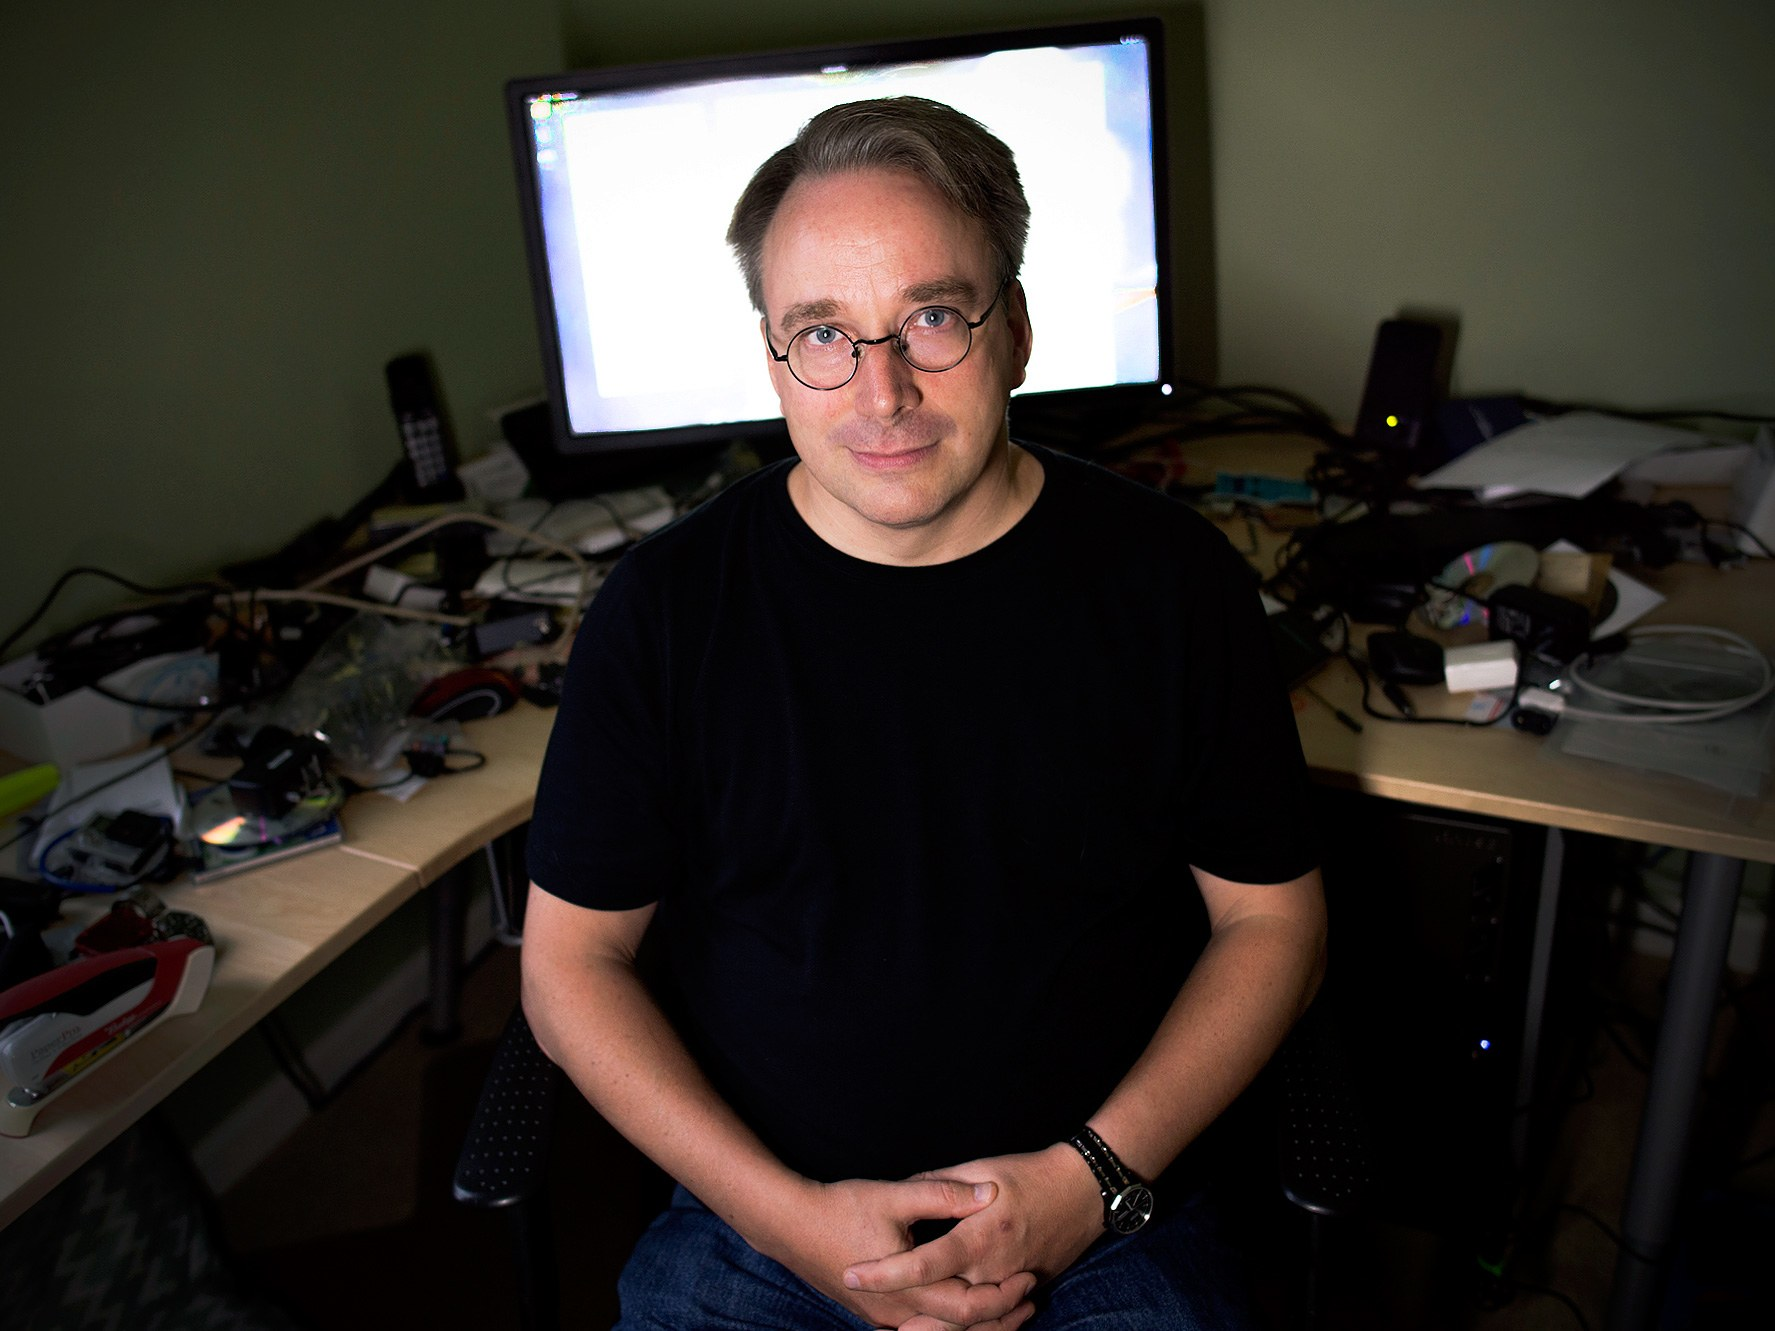
\includegraphics[width=\textwidth]{figures/linus.jpg}
            \end{figure}
        \end{columns}
    \end{frame}

    \section{GitHub}\label{sec:github}
    \begin{frame}{GitHub}
        \begin{columns}
            \column{0.5\textwidth}
            \begin{itemize}
                \item \url{https://github.com/}
                \item Central repository sharing
                \item Public and private options
                \item Project management
            \end{itemize}

            \column{0.5\textwidth}
            \begin{figure}
                \centering
                
\includegraphics[width=\textwidth]{figures/Octocat.png}
            \end{figure}
        \end{columns}

        \begin{alertblock}{Be mindful of privacy!}
            Never store sensitive information in git! There are better solutions for managing passwords, encryption keys, or other sensitive information.
        \end{alertblock}
    \end{frame}

    \begin{frame}{Creating an Account}
        Navigate to \url{https://github.com/}

        \begin{figure}
            \centering
            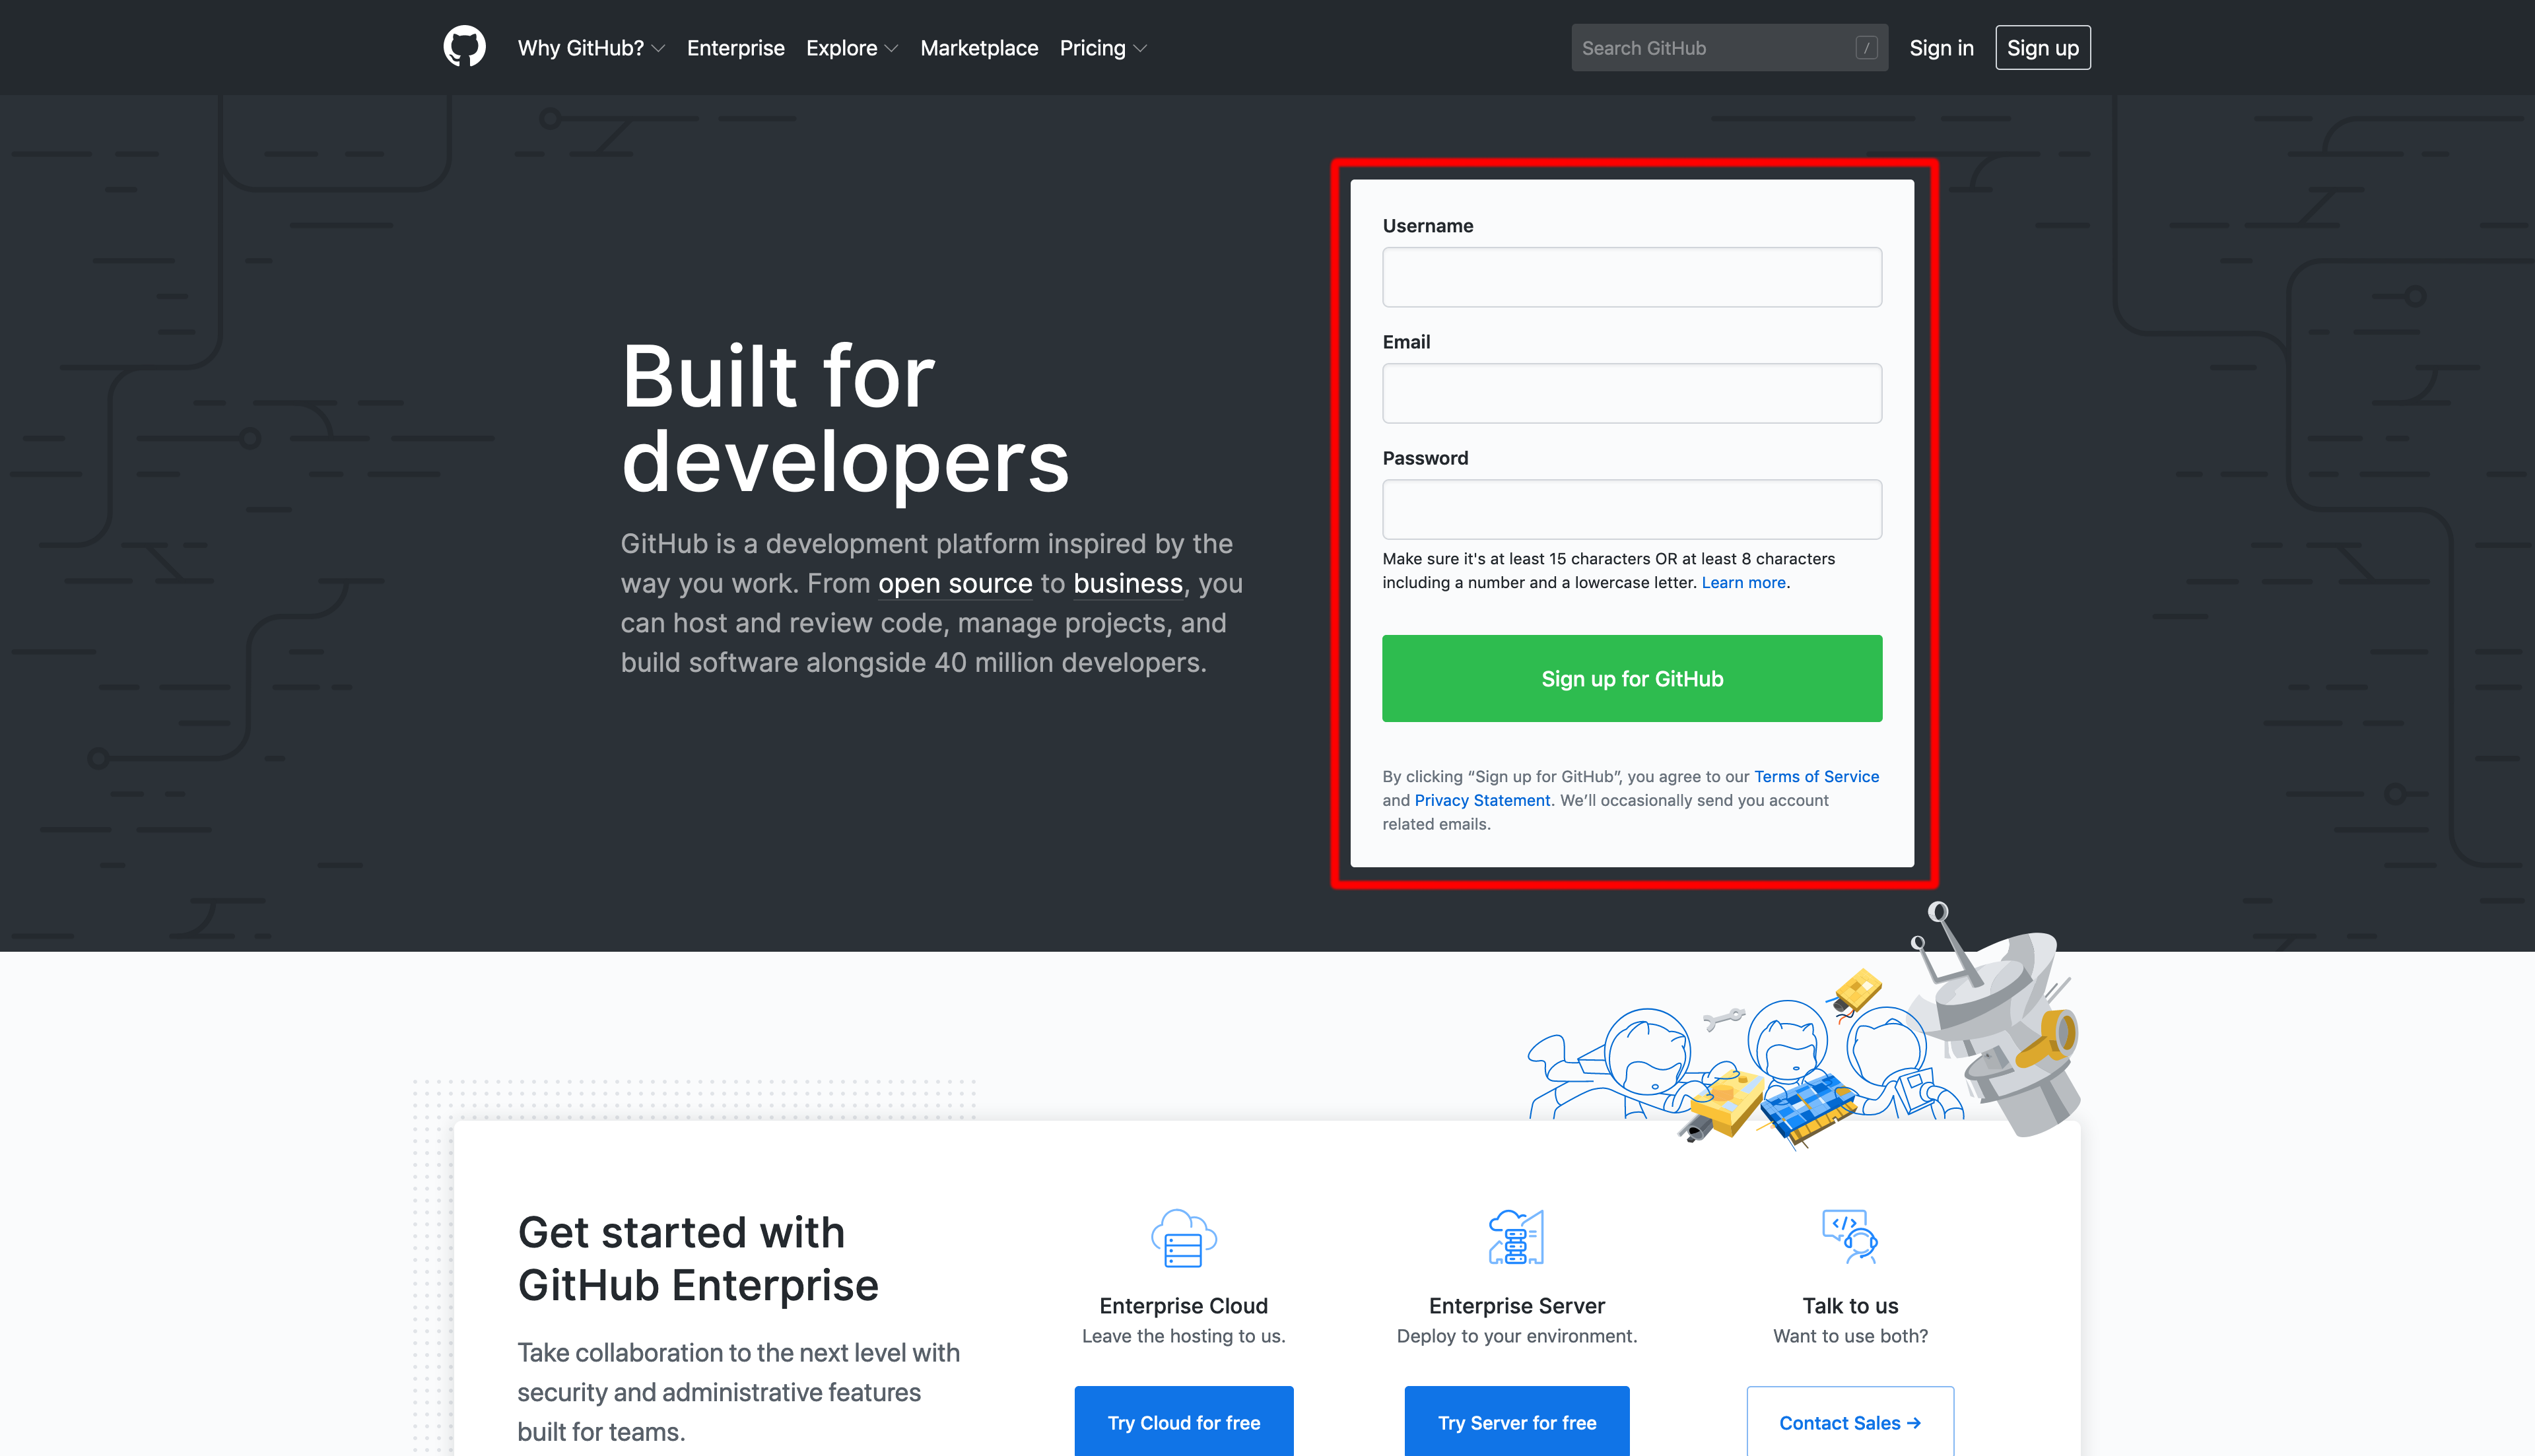
\includegraphics[width=\textwidth]{figures/github.png}
        \end{figure}
    \end{frame}

    \begin{frame}{Creating a Repository}
        After logging into GitHub\ldots
        \begin{columns}
            \column{0.5\textwidth}
            \begin{figure}
                \centering
                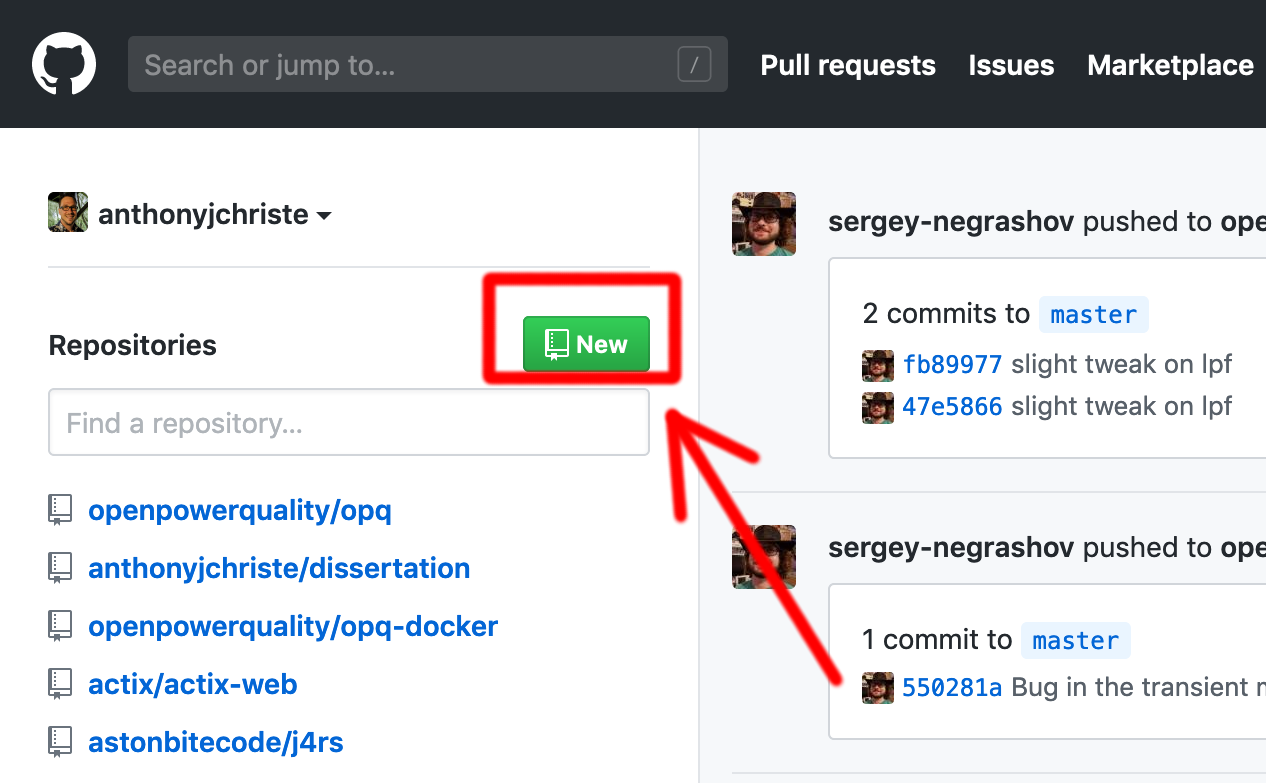
\includegraphics[width=\textwidth]{figures/github_new_1.png}
            \end{figure}

            \column{0.5\textwidth}
            \begin{figure}
                \centering
                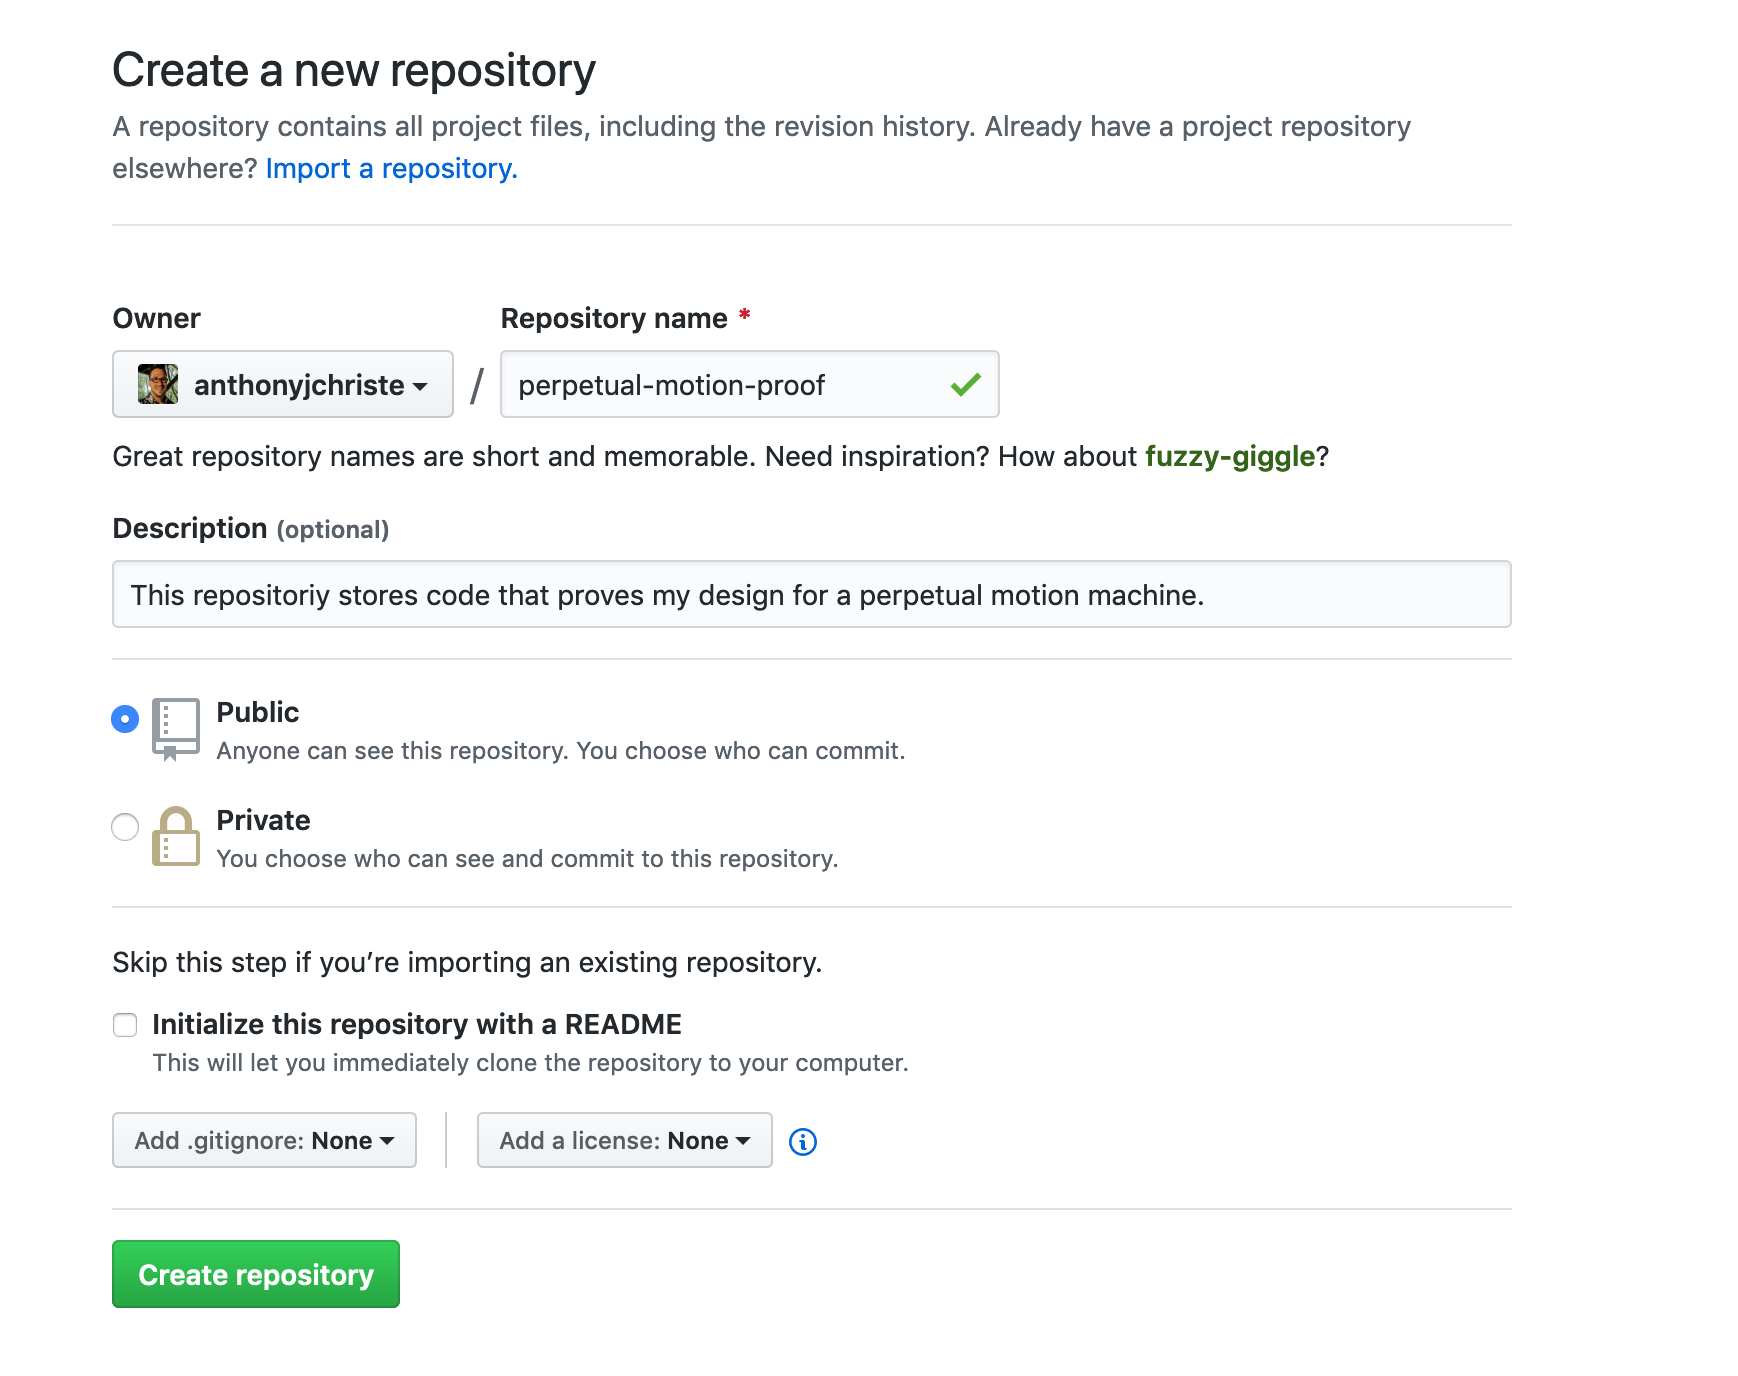
\includegraphics[width=\textwidth]{figures/github_new_2.png}
            \end{figure}

        \end{columns}
    \end{frame}

    \section{An Interlude on git Terminology}
    \begin{frame}{Common git Terminology}
        General workflow
        \begin{itemize}
            \item clone - Copy history of remote repo
            \item pull - Update changes from remote to local repo
            \item add - Stage changes to local repo
            \item commit - Commit changes to local repo
            \item push - Push changes to remote repo
        \end{itemize}

        Less general, but still useful
        \begin{itemize}
            \item merge - Merge multiple changes
            \item branches -
            \item pull request - Review of changes before merging into master branch
        \end{itemize}
    \end{frame}

    \section{GitHub Desktop}
    \begin{frame}{GitHub Desktop}
        \begin{columns}
            \column{0.3\textwidth}
            \begin{itemize}
                \item GUI for git
                \item Cross-platform
                \item Open-source
            \end{itemize}

            \column{0.7\textwidth}
            \begin{figure}
                \centering
                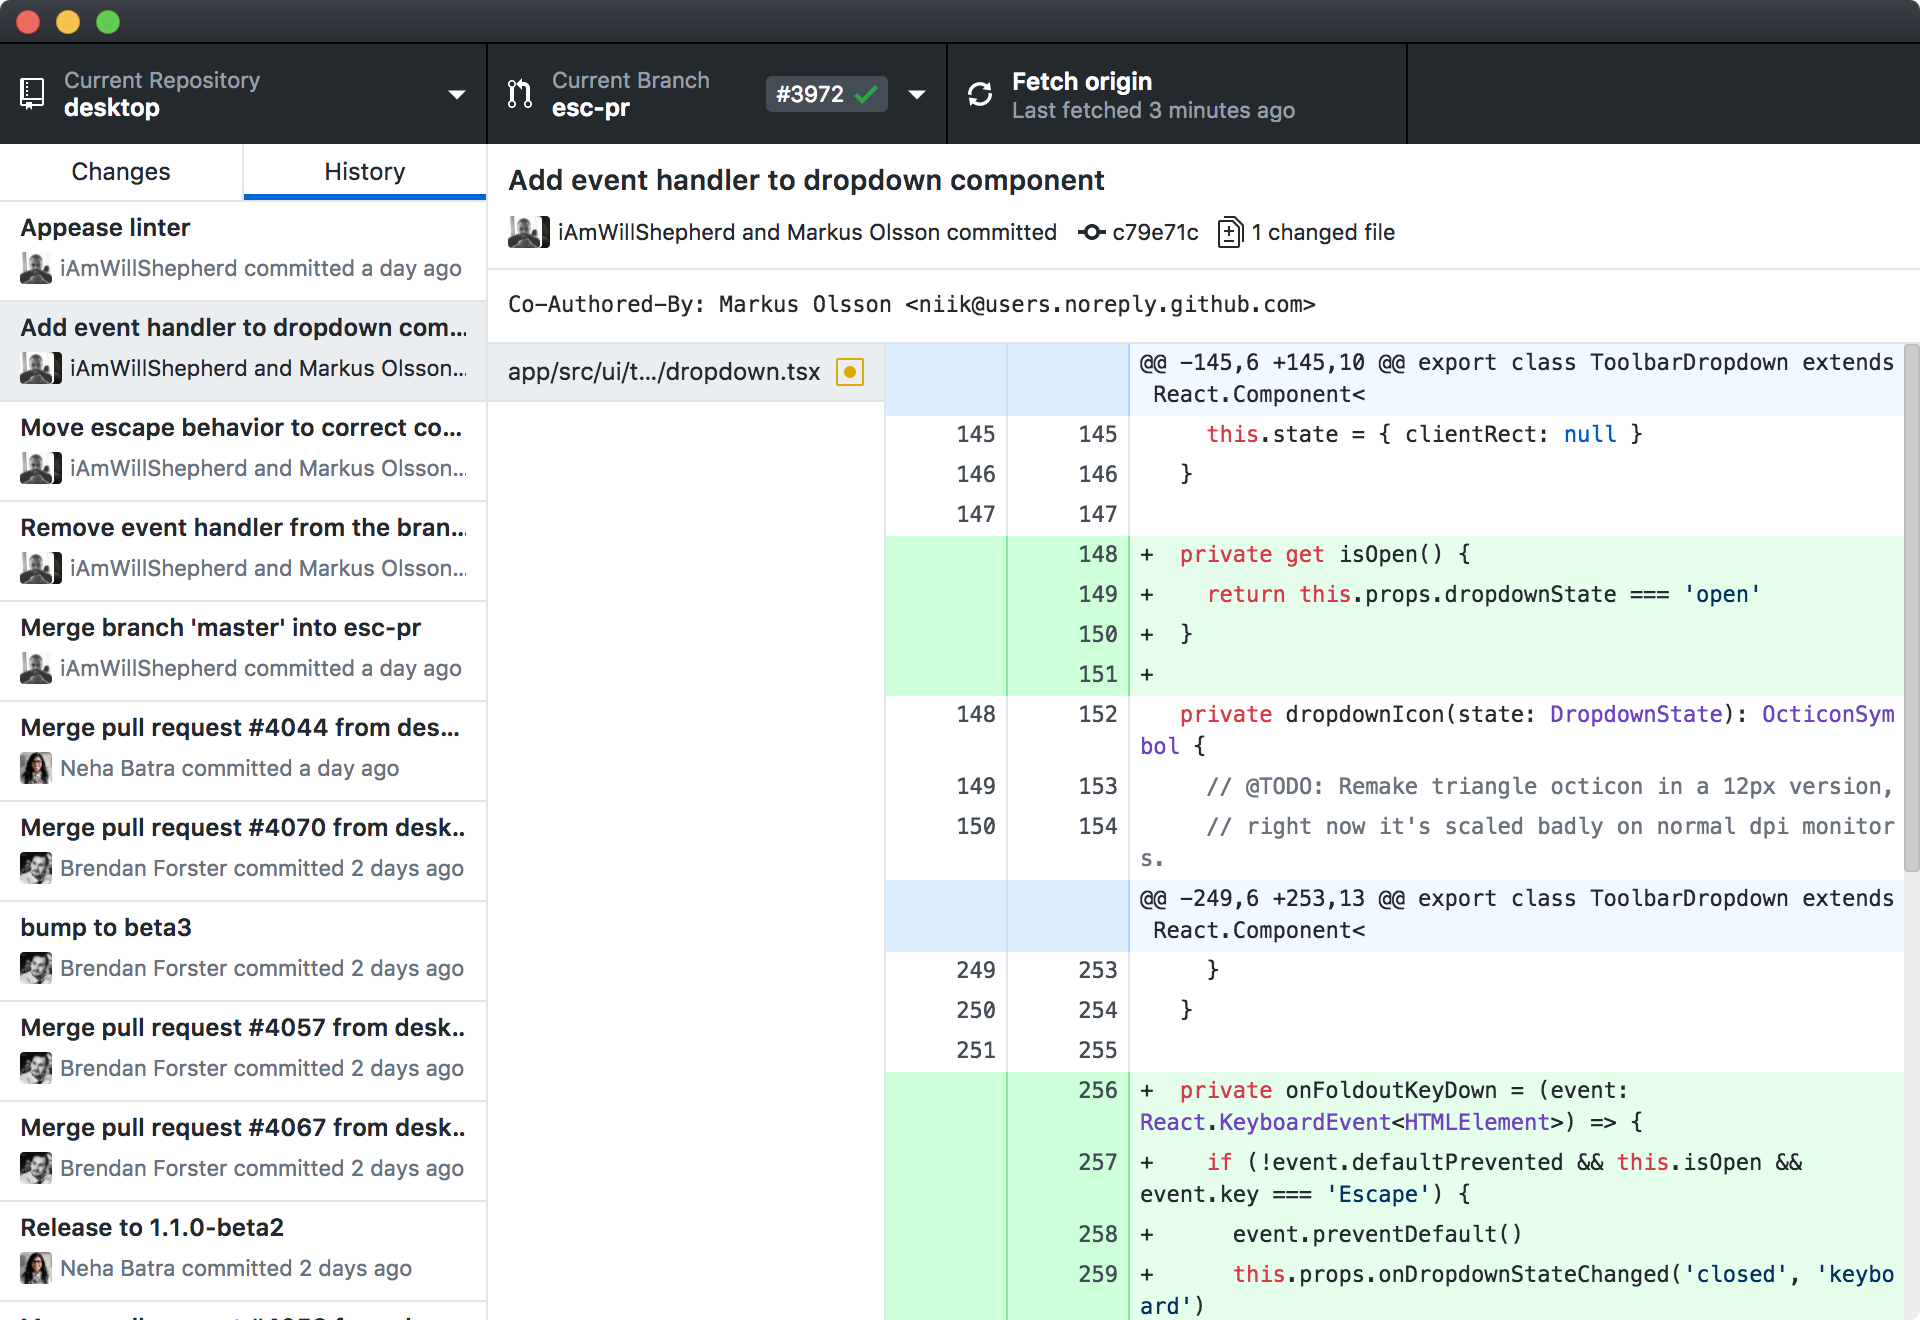
\includegraphics[width=\textwidth]{figures/github-desktop-screenshot-mac.png}
            \end{figure}
        \end{columns}
        \centering
        \url{https://desktop.github.com/}

        \url{https://help.github.com/en/desktop/getting-started-with-github-desktop/setting-up-github-desktop}
    \end{frame}

    \begin{frame}{Don't Fear the CLI}
        GitHub Desktop makes it easy to manage git repositories. That said, it is useful to play around with and understand git's Command Line Interface (CLI).
        \begin{itemize}
            \item You're on a platform that doesn't support GitHub Desktop
            \item You're SSHed into a server somewhere
            \item Most git related solutions on Google and Stack Overflow use the CLI
        \end{itemize}
    \end{frame}

    \section{Cloning a Respository}
    \begin{frame}{Cloning a Repository}
        \begin{columns}
            \column{0.5\textwidth}
            \begin{itemize}
                \item Open GitHub Desktop
                \item Log-In / Configure
                \item Clone
            \end{itemize}

            \column{0.5\textwidth}
            \begin{figure}
                \centering
                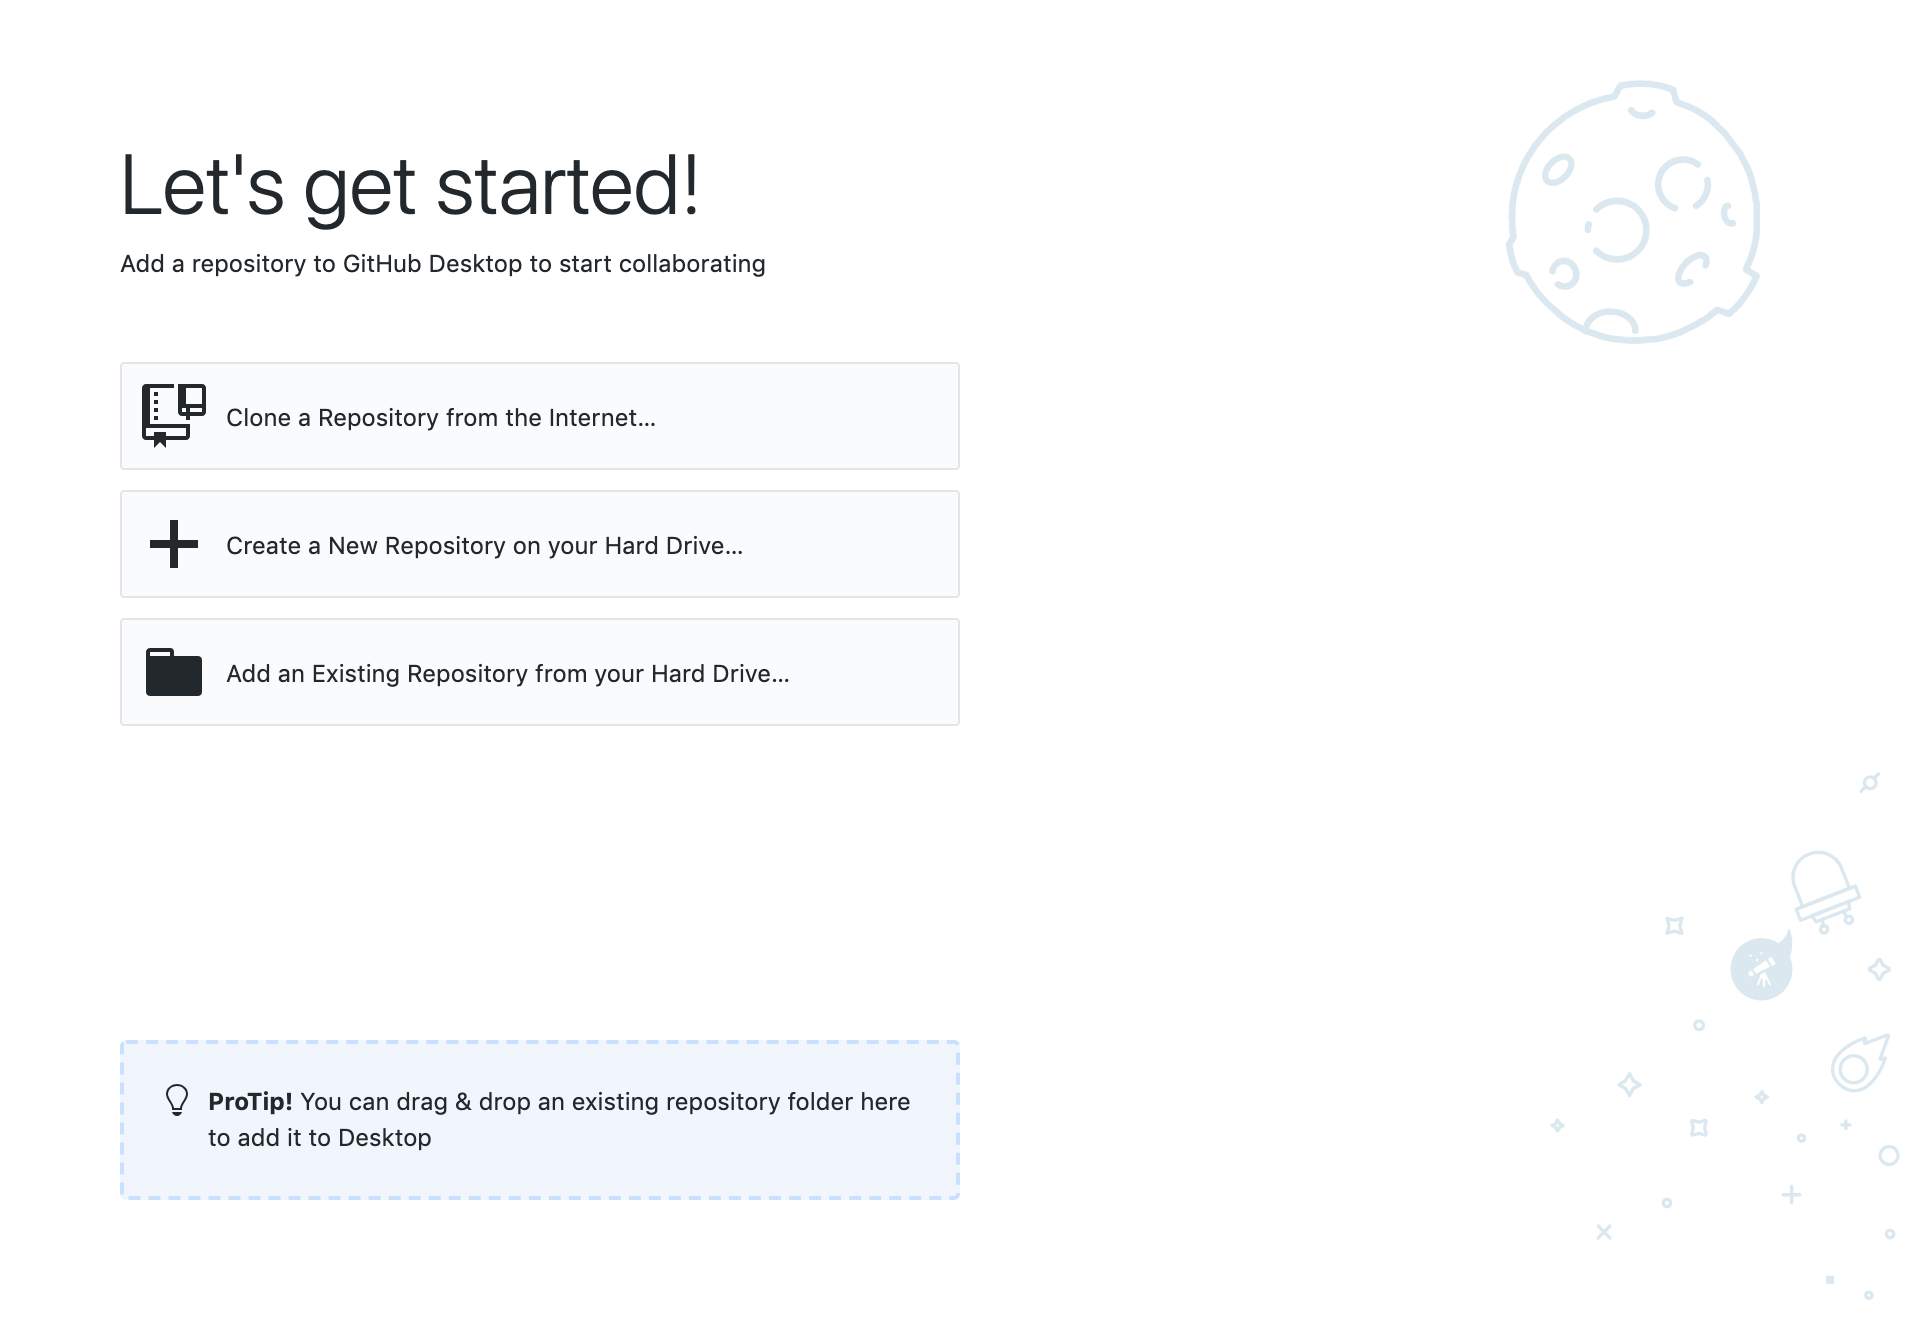
\includegraphics[width=\textwidth]{figures/clone_1.png}
            \end{figure}
        \end{columns}
    \end{frame}

    \begin{frame}{Cloning a Repository}
        \begin{columns}
            \column{0.5\textwidth}
            \begin{figure}
                \centering
                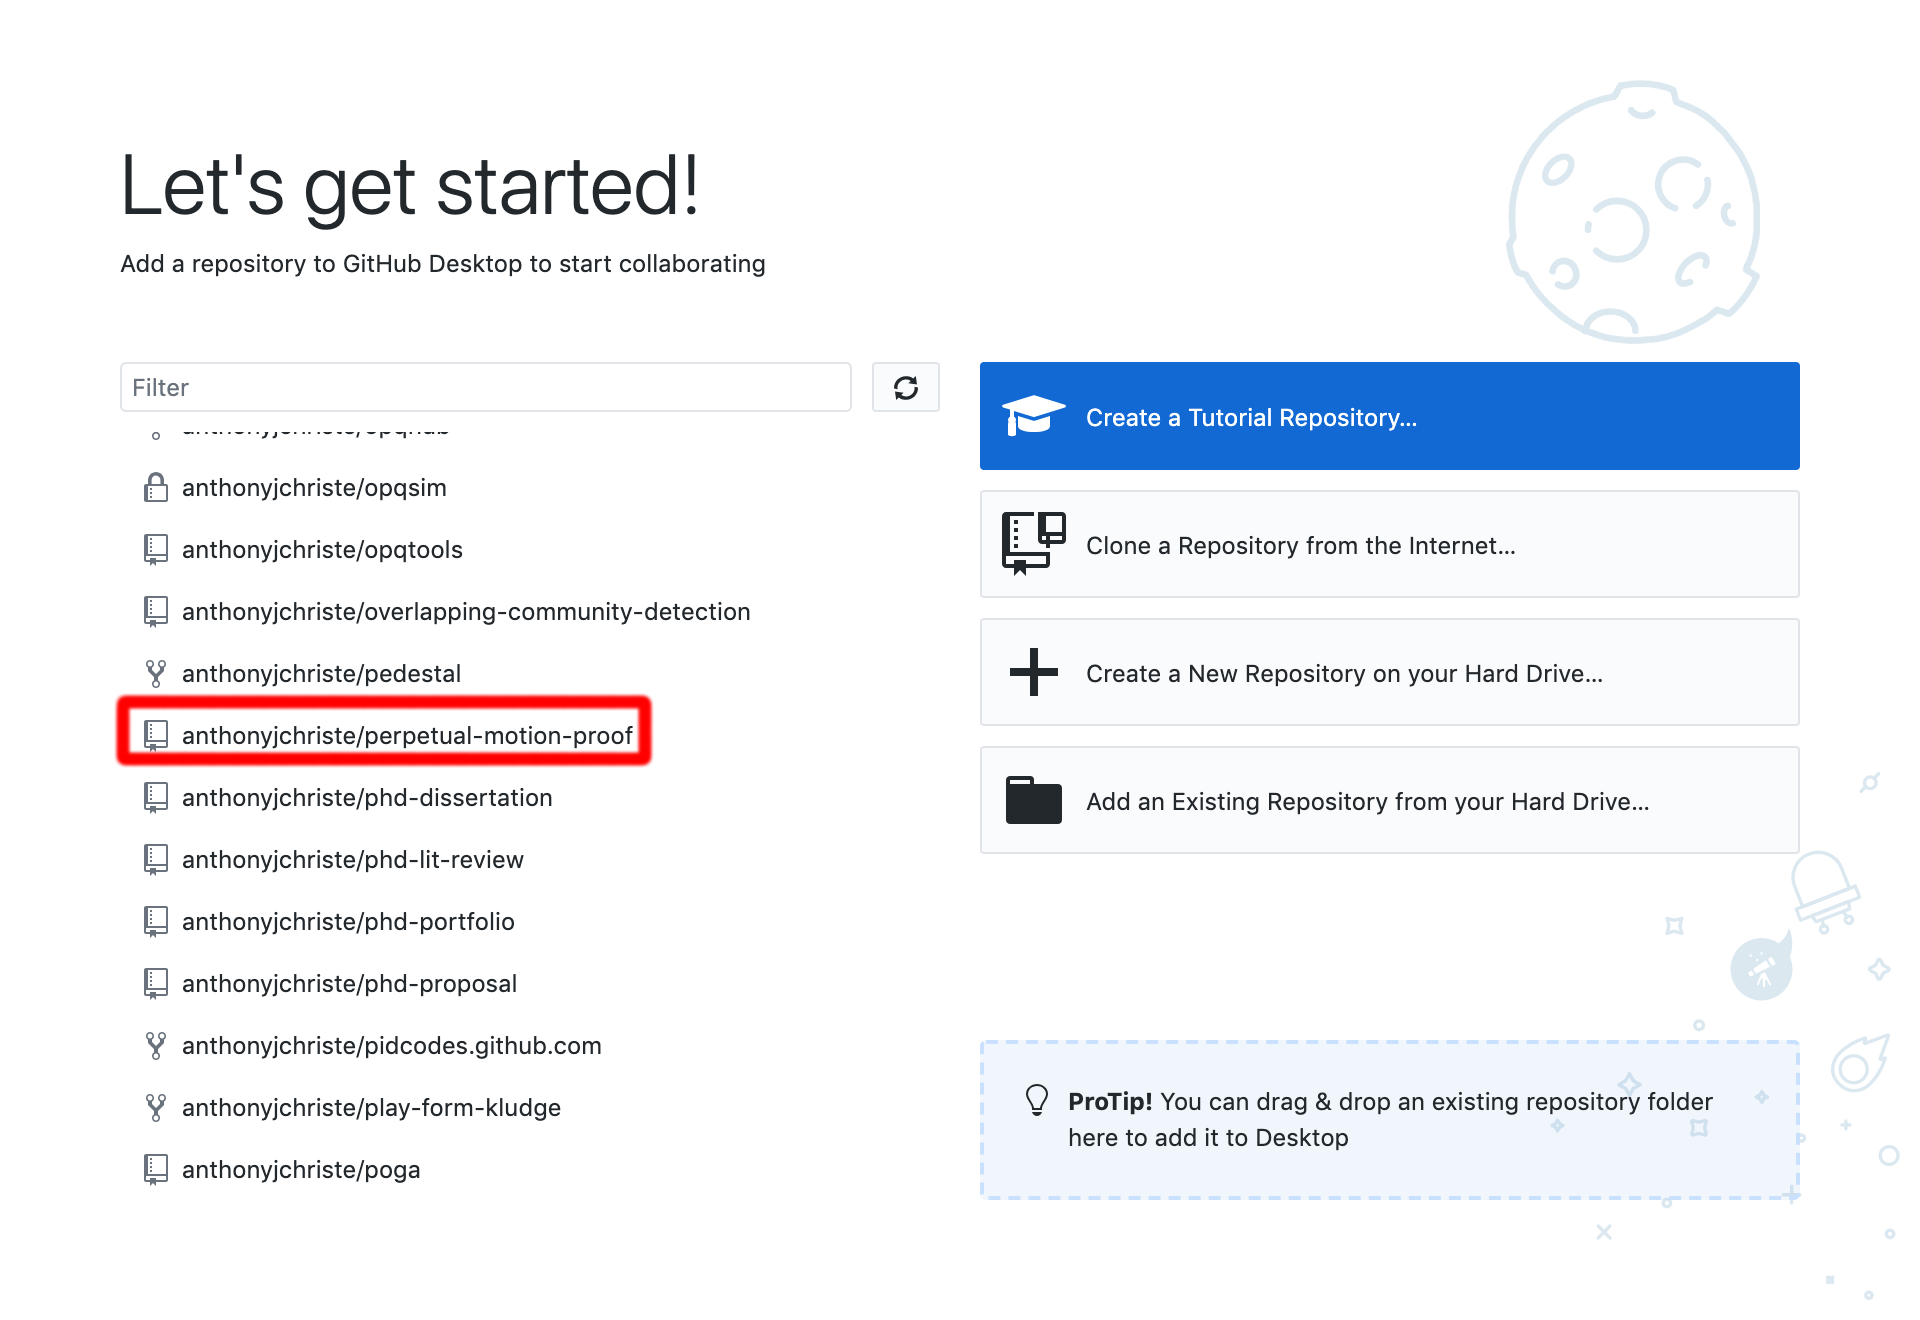
\includegraphics[width=\textwidth]{figures/clone_2.png}
            \end{figure}

            \column{0.5\textwidth}
            \begin{figure}
                \centering
                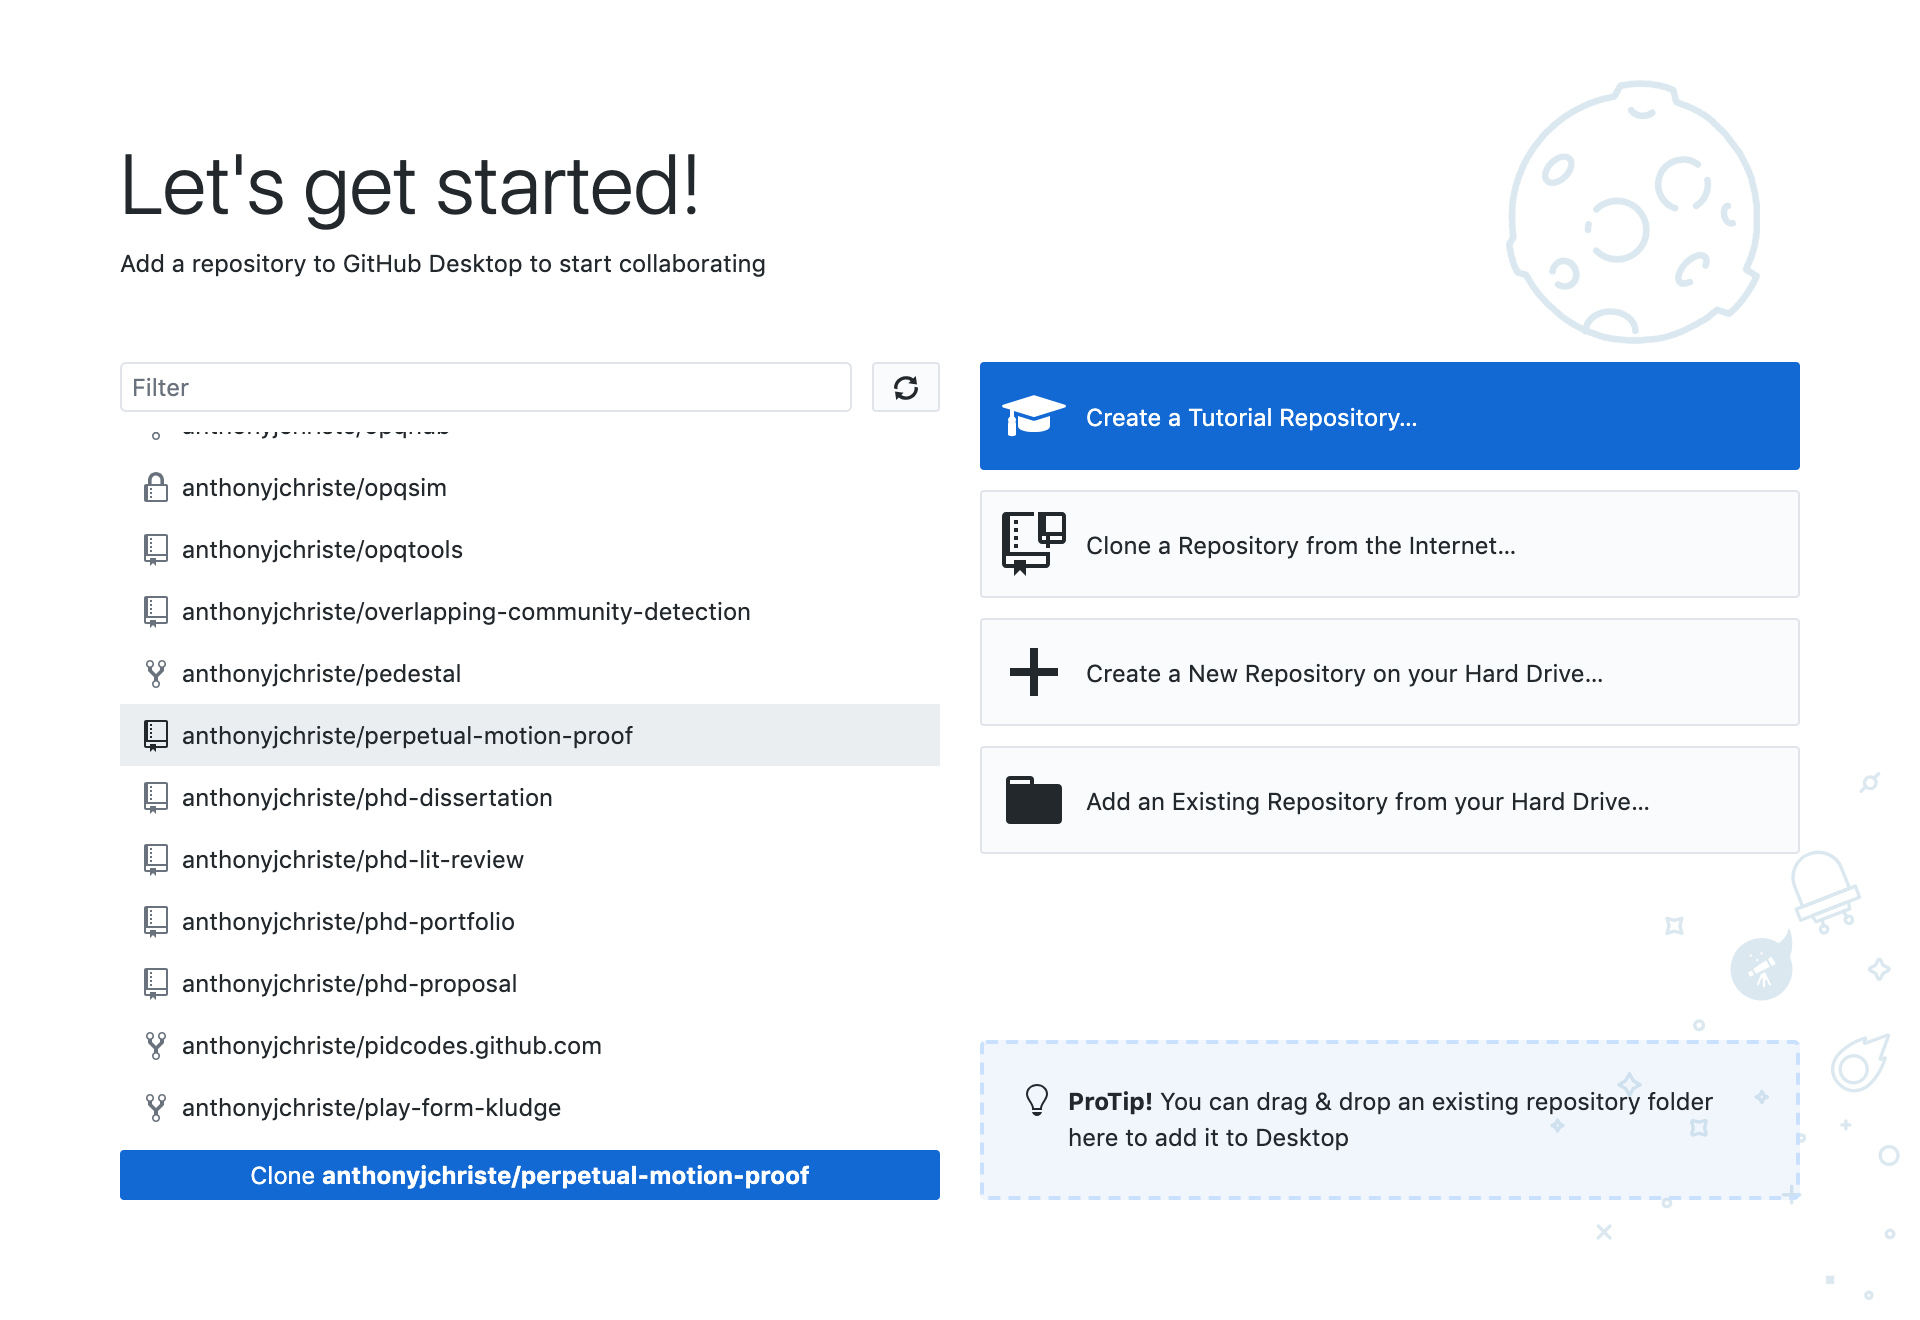
\includegraphics[width=\textwidth]{figures/clone_3.png}
            \end{figure}
        \end{columns}
    \end{frame}

    \begin{frame}{Cloning a Repository}
        \begin{columns}
            \column{0.5\textwidth}
            \begin{figure}
                \centering
                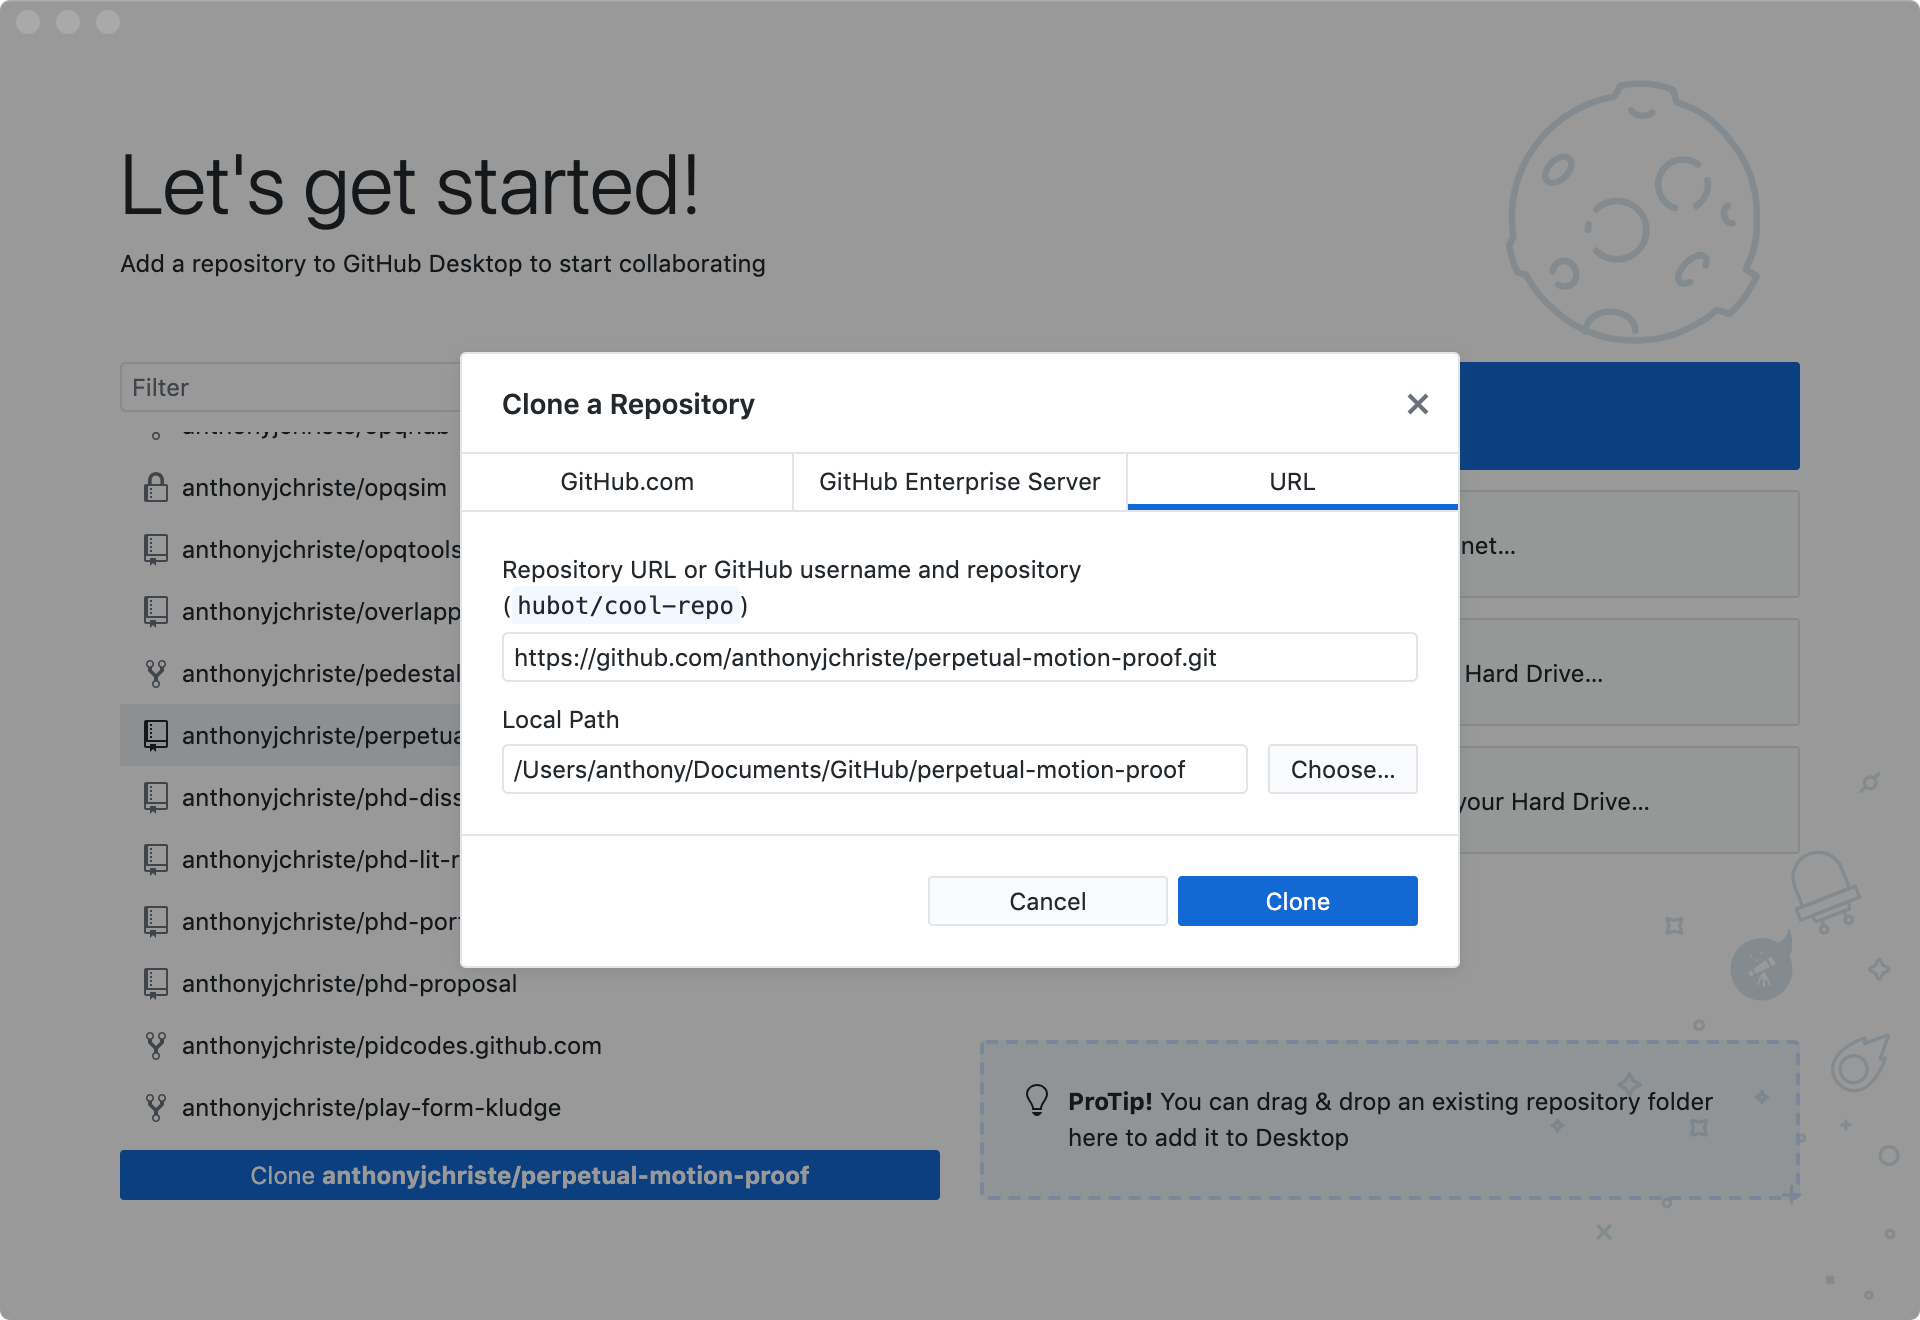
\includegraphics[width=\textwidth]{figures/clone_4.png}
            \end{figure}

            \column{0.5\textwidth}
            \begin{figure}
                \centering
                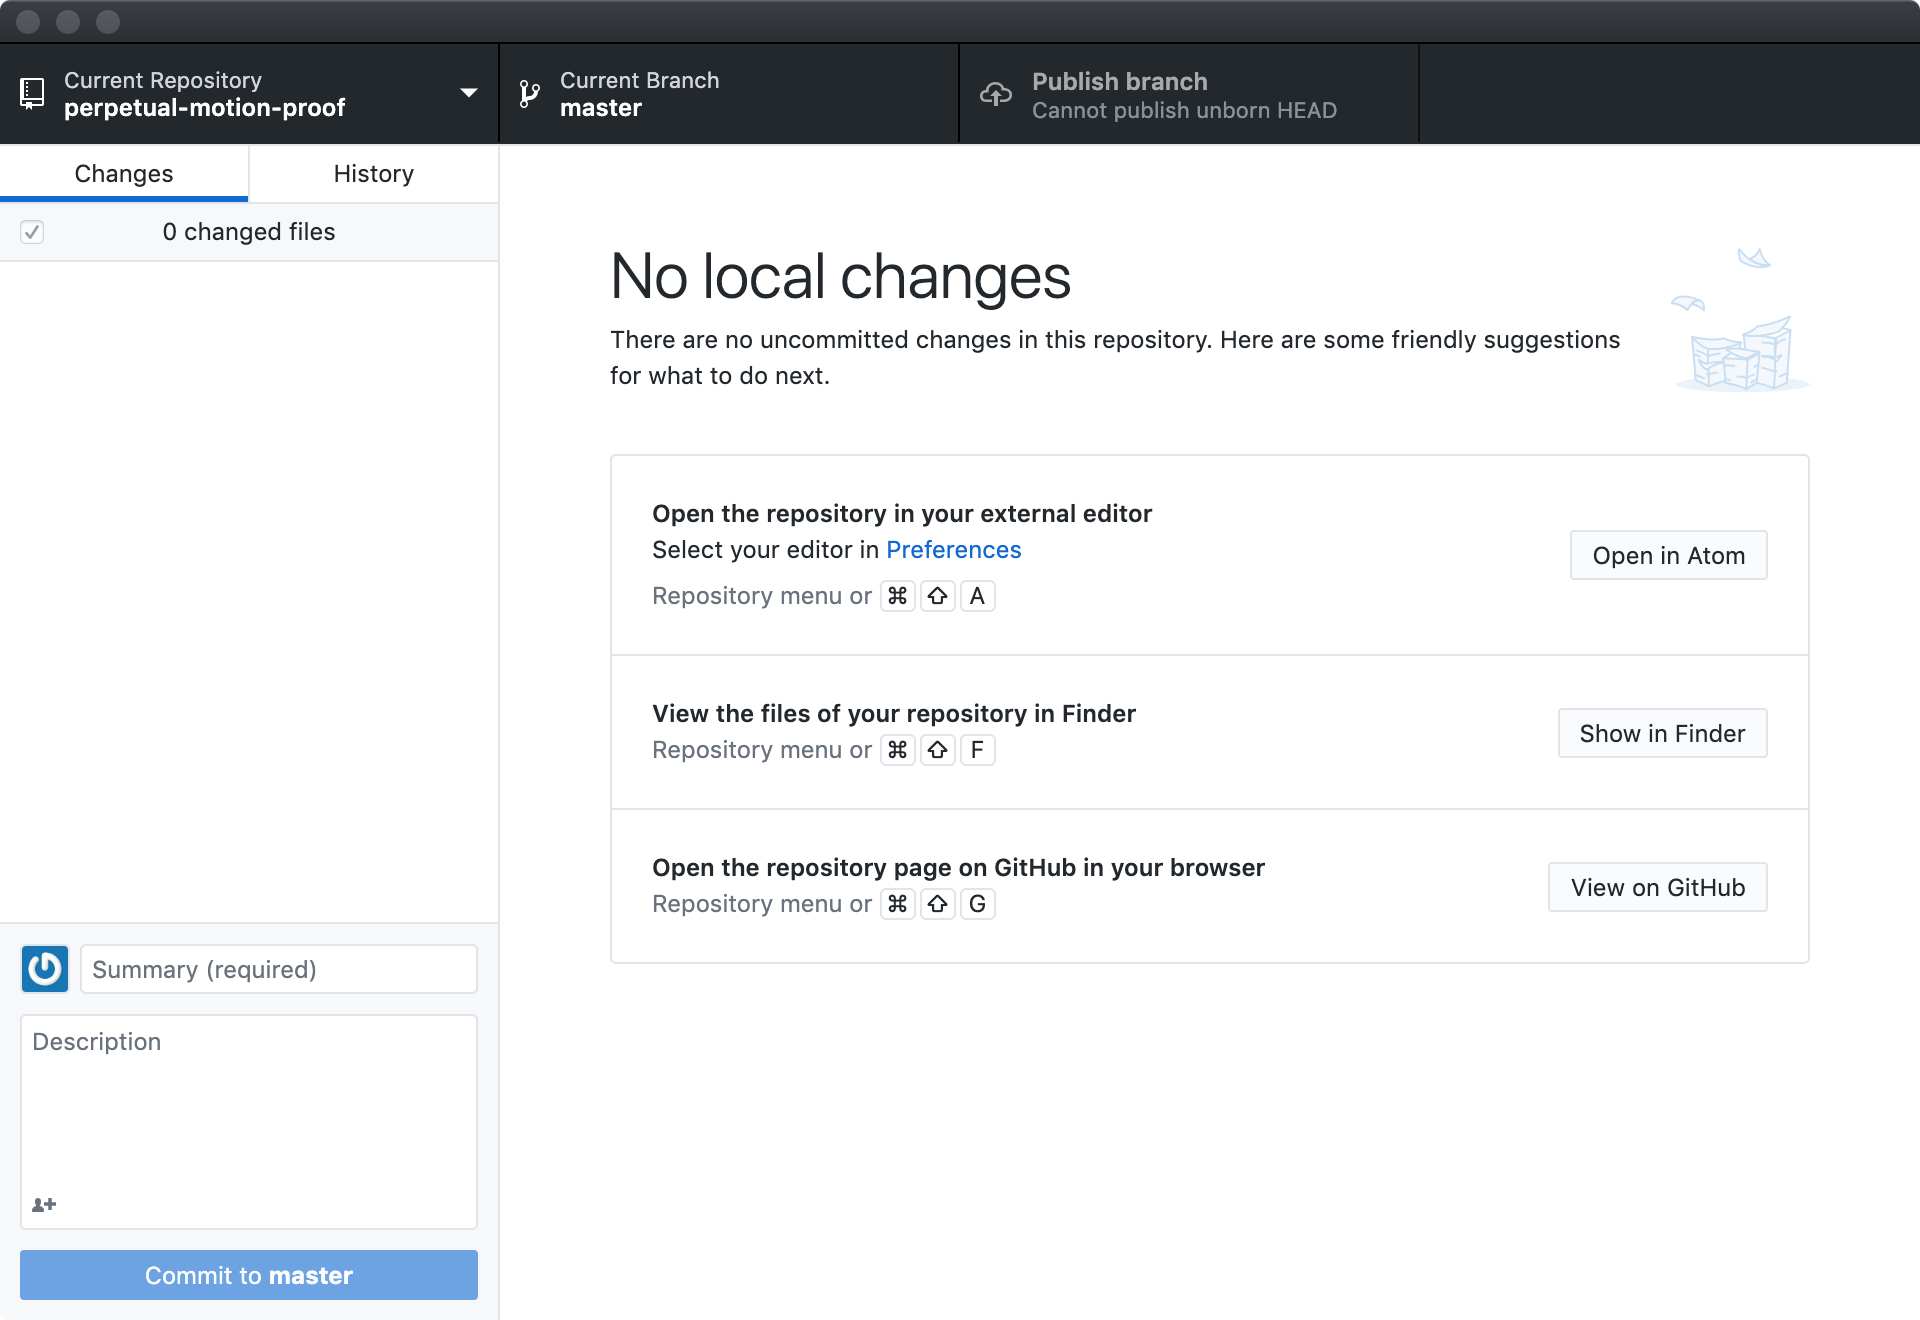
\includegraphics[width=\textwidth]{figures/clone_5.png}
            \end{figure}
        \end{columns}
    \end{frame}

%    \begin{frame}{Upload an Existing Repository}
%    \end{frame}

    \section{Add, commit, \& push changes}
    \begin{frame}{Adding Changes}
        First, add a ``README.md" file.
        \begin{itemize}
            \item Add a project description
            \item Commit the changes
            \item Push the changes
        \end{itemize}

        Next, add a ``pmotion.py" file
        \begin{itemize}
            \item Add the code
            \item Commit the changes
            \item Push the changes
        \end{itemize}
    \end{frame}

    \begin{frame}{Adding Changes (README.md)}
        \begin{figure}
            \centering
            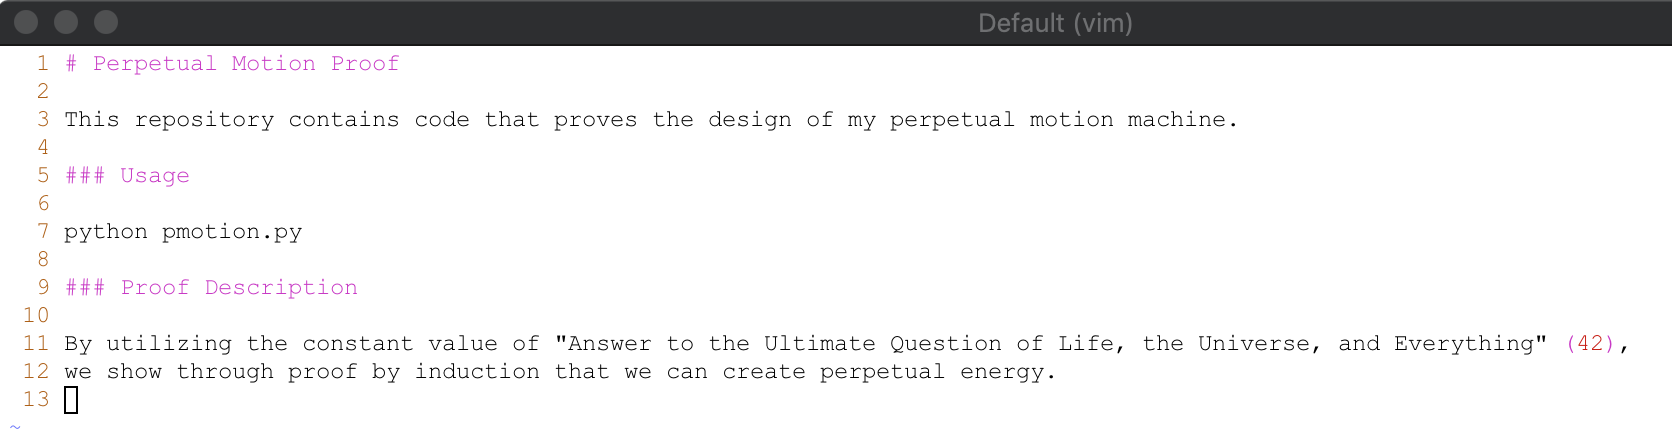
\includegraphics[width=\textwidth]{figures/add_1.png}
        \end{figure}
        \centering
        Add the project description
    \end{frame}

    \begin{frame}{Adding Changes (README.md)}
        \begin{figure}
            \centering
            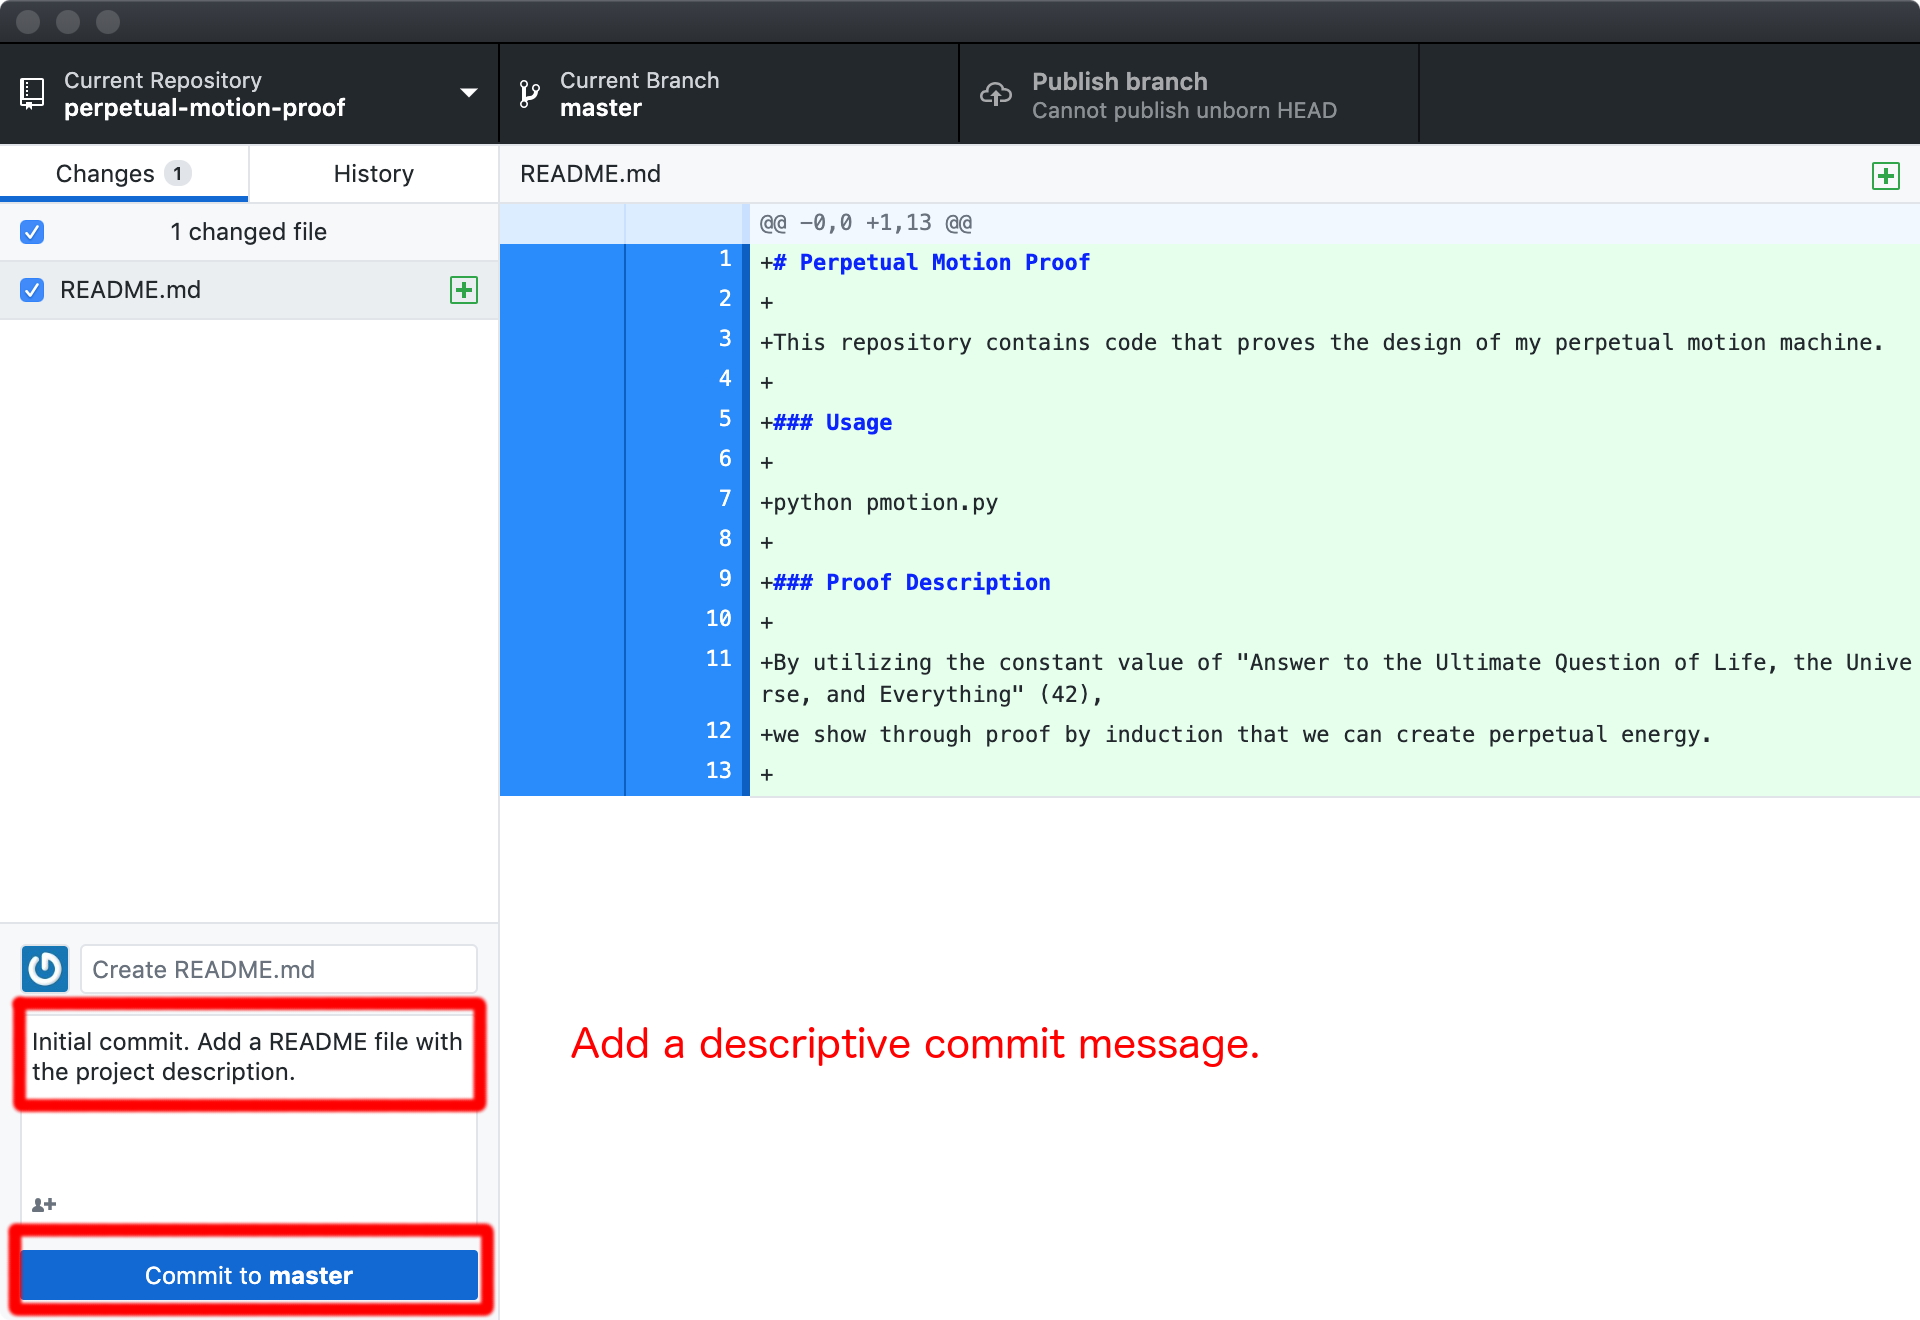
\includegraphics[width=0.8\textwidth]{figures/add_2.png}
        \end{figure}

        \centering
        Commit the changes
    \end{frame}

    \begin{frame}{Adding Changes (README.md)}
        \begin{figure}
            \centering
            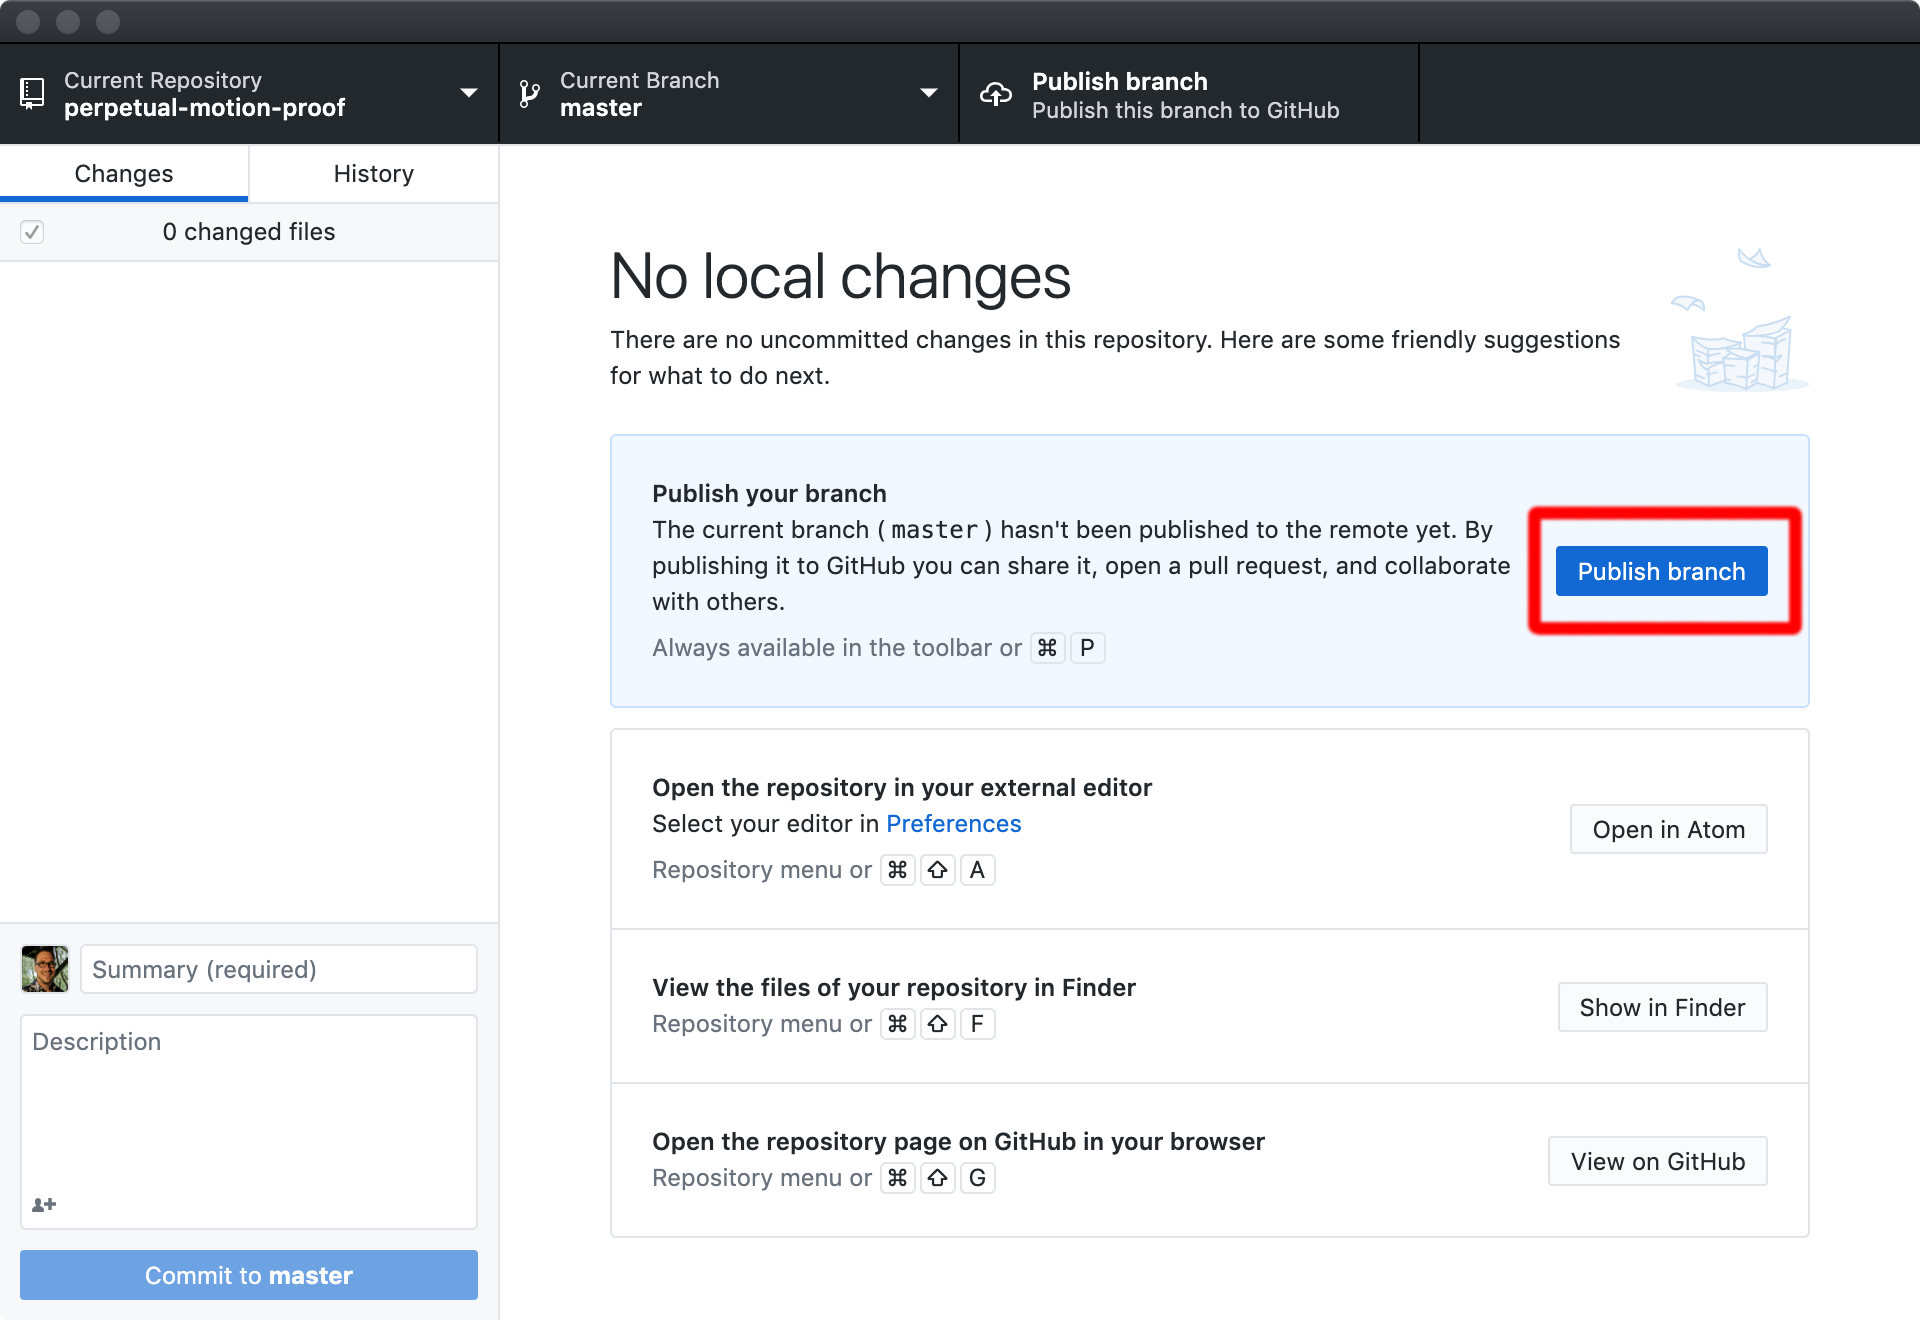
\includegraphics[width=0.8\textwidth]{figures/add_3.png}
        \end{figure}

        \centering
        Push the changes
    \end{frame}

    \begin{frame}{Adding Changes (pmotion.py)}
        \begin{figure}
            \centering
            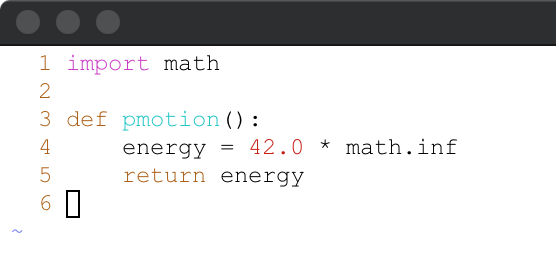
\includegraphics[width=\textwidth]{figures/add_4.png}
        \end{figure}
        \centering
        Add the code
    \end{frame}

    \begin{frame}{Adding Changes (pmotion.py)}
        \begin{figure}
            \centering
            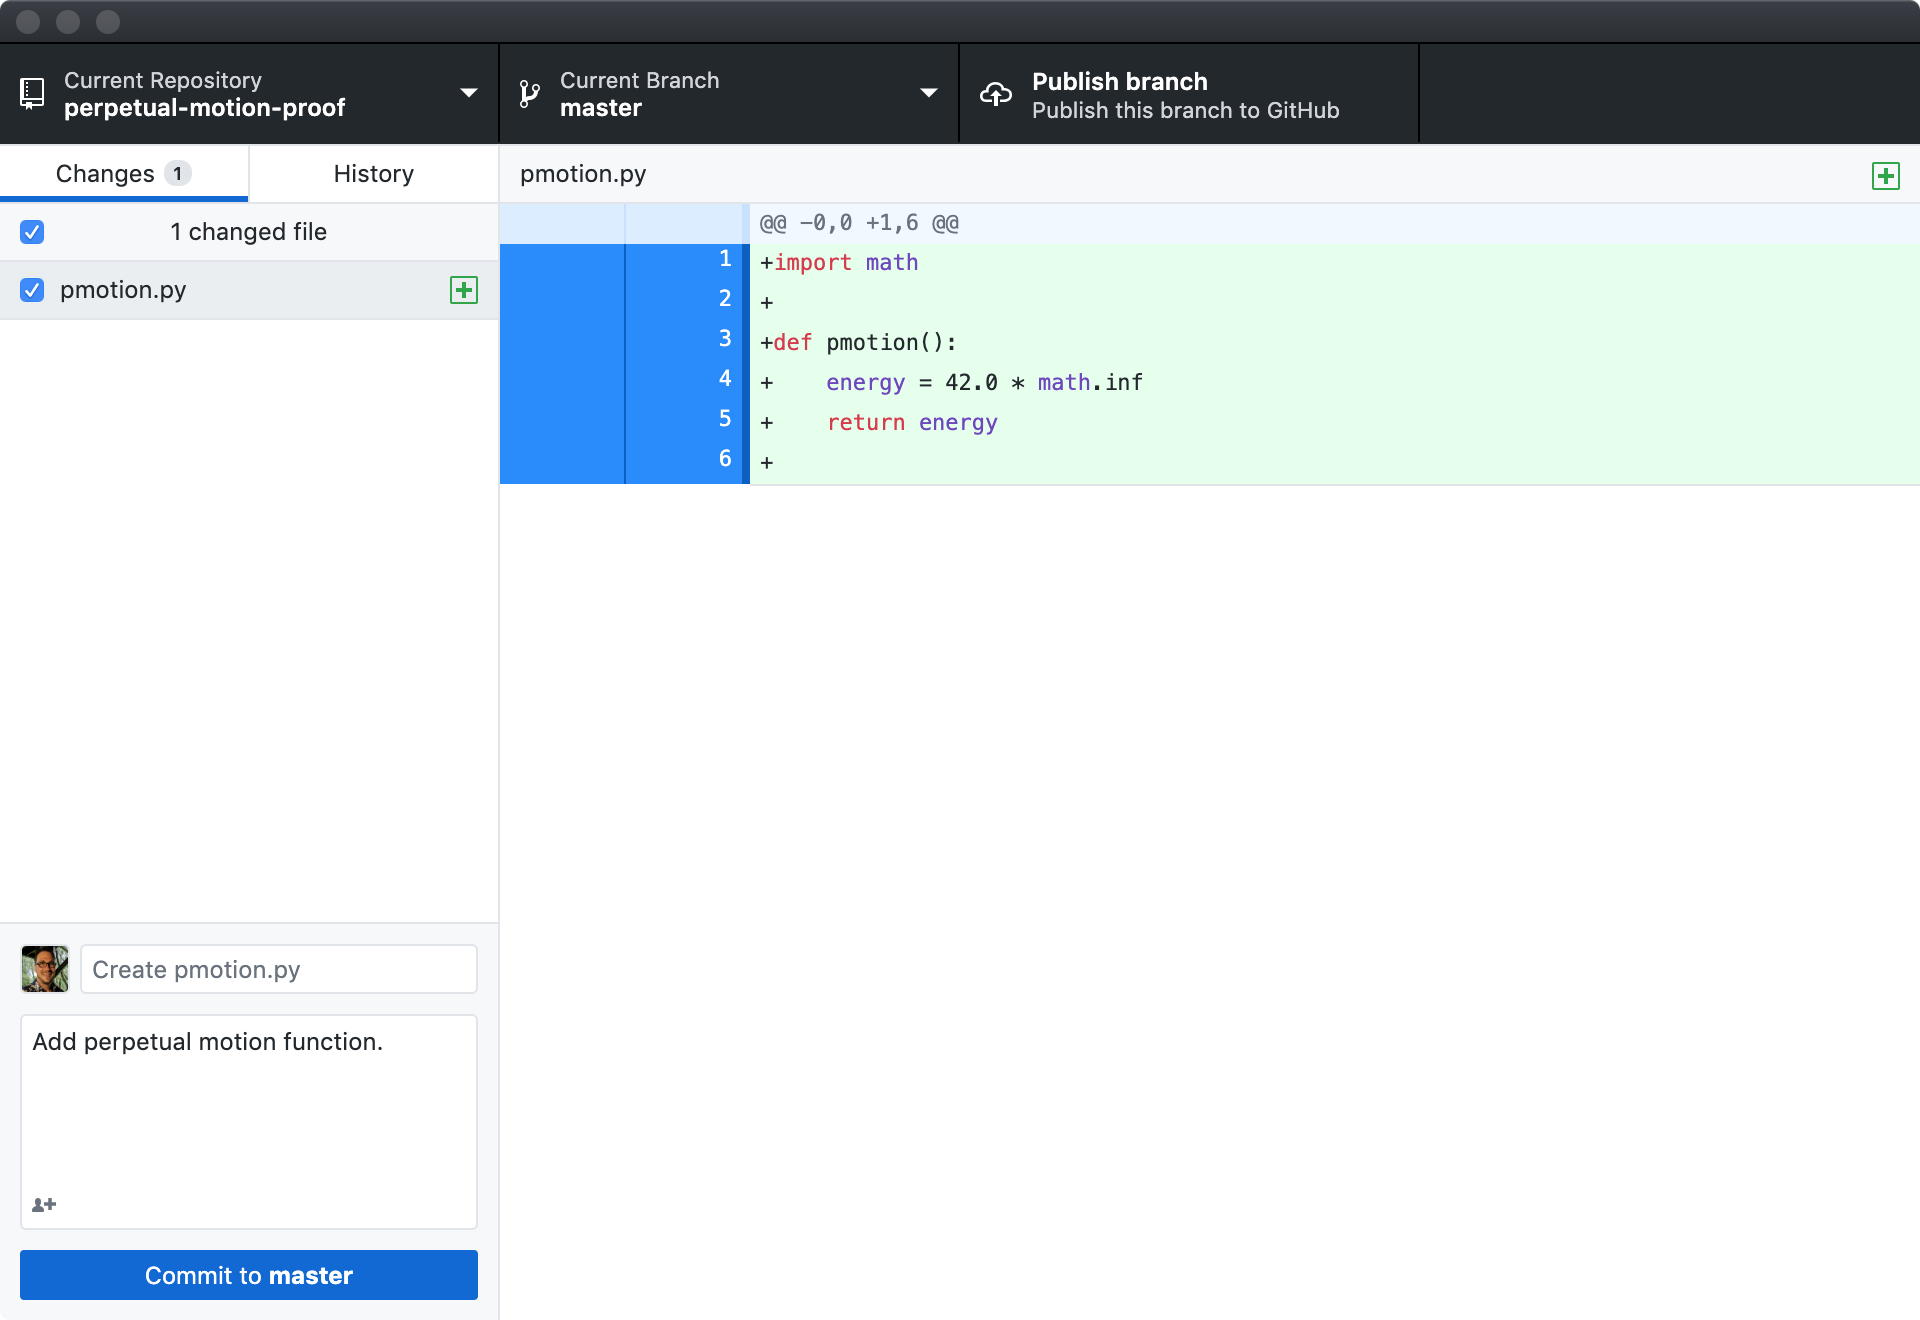
\includegraphics[width=0.8\textwidth]{figures/add_5.png}
        \end{figure}

        \centering
        Commit the changes
    \end{frame}

    \begin{frame}{Adding Changes (pmotion.py)}
        \begin{figure}
            \centering
            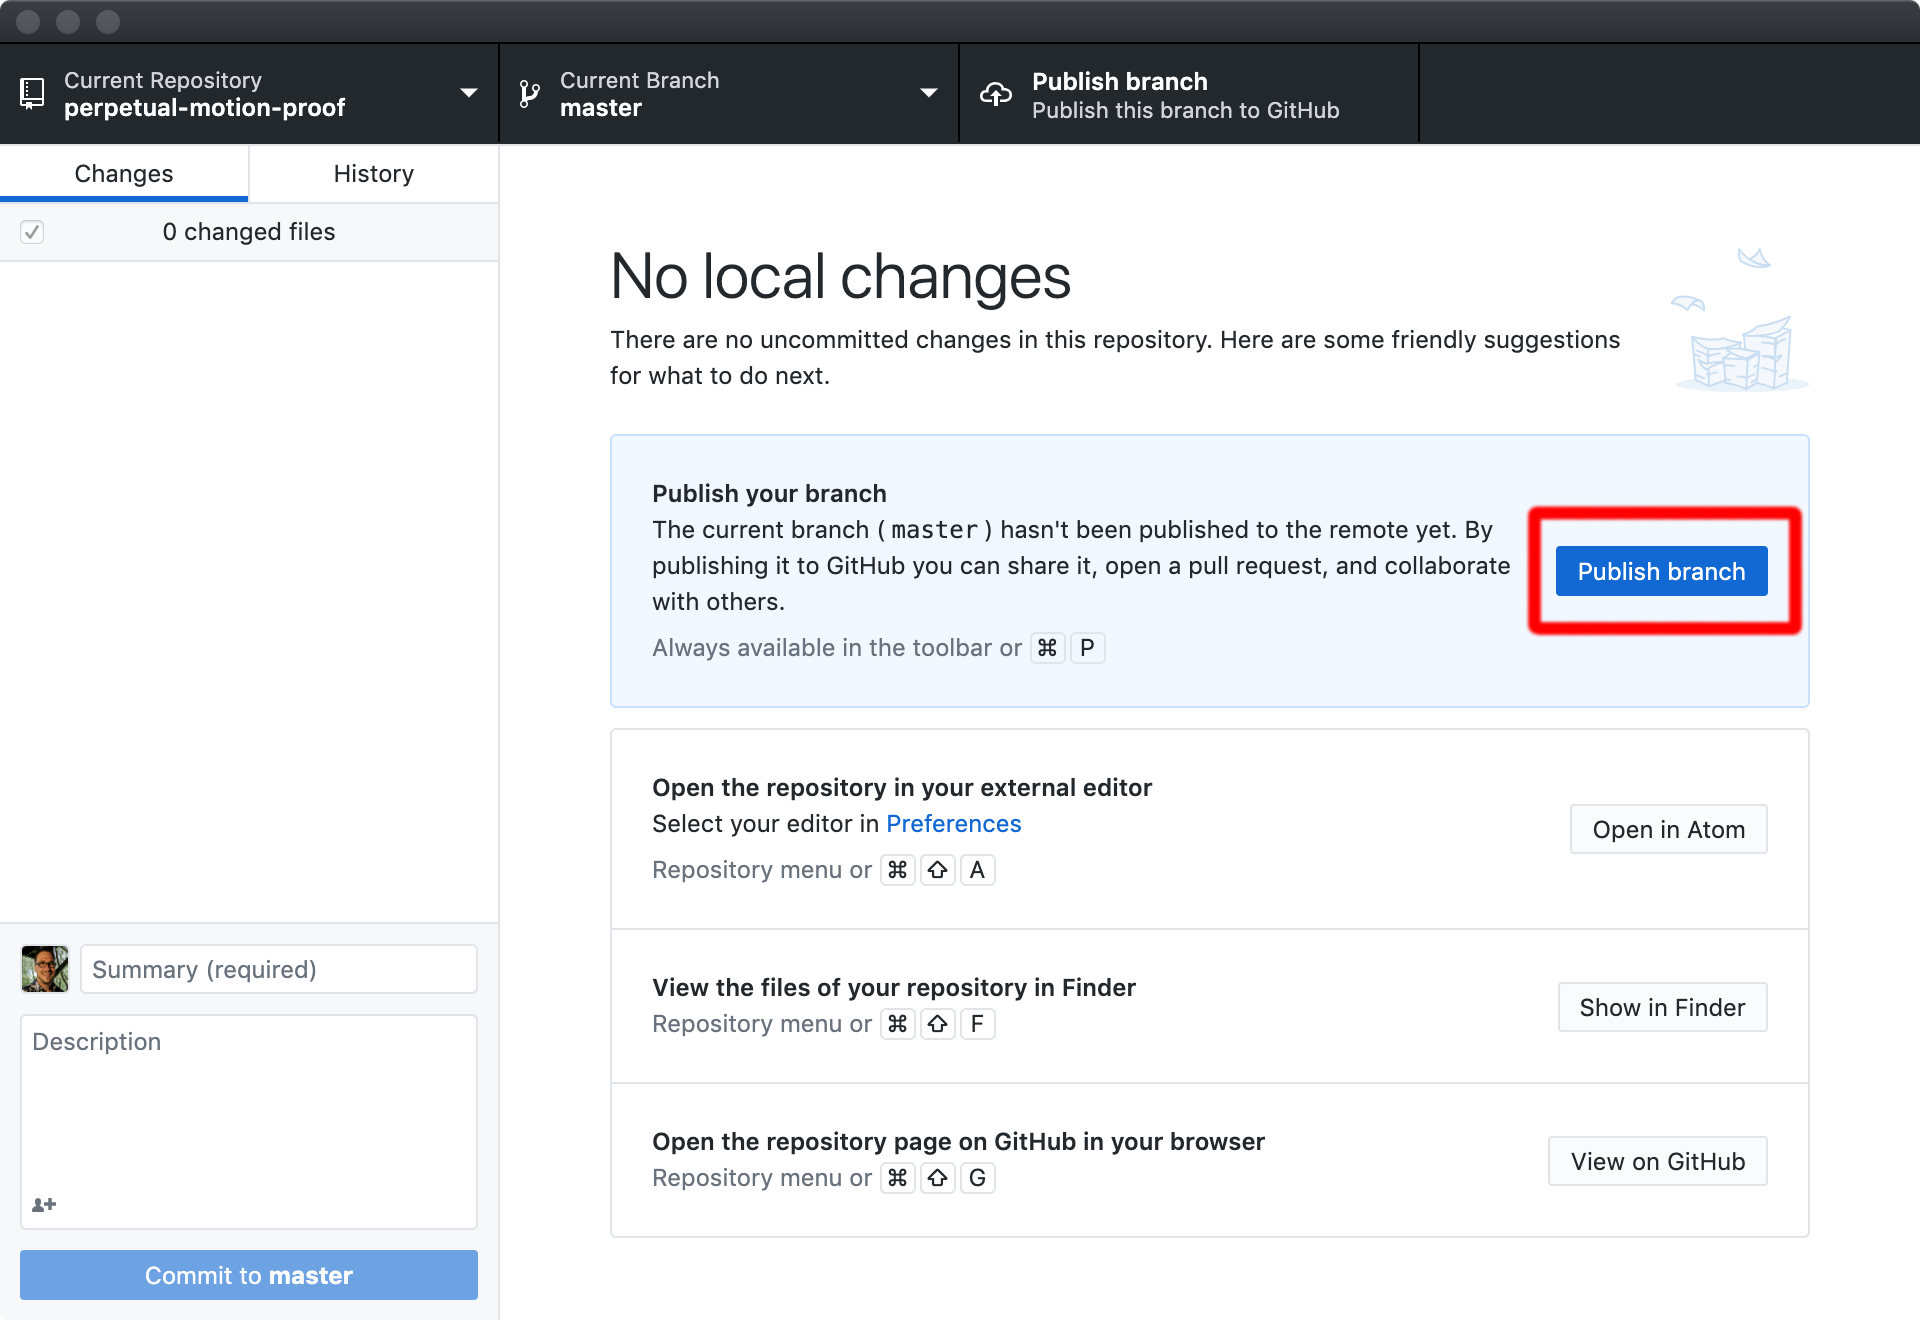
\includegraphics[width=0.8\textwidth]{figures/add_3.png}
        \end{figure}

        \centering
        Push the changes
    \end{frame}

    \begin{frame}{Fetching/Pulling Changes}
            \begin{itemize}
                \item Someone makes changes to your code
                \item They push their changes to GitHub
                \item ``fetch" and ``pull" to get their changes
            \end{itemize}
    \end{frame}

    \begin{frame}{Fetching/Pulling Changes}
        \begin{columns}
            \column{0.5\textwidth}
            \begin{figure}
                \centering
                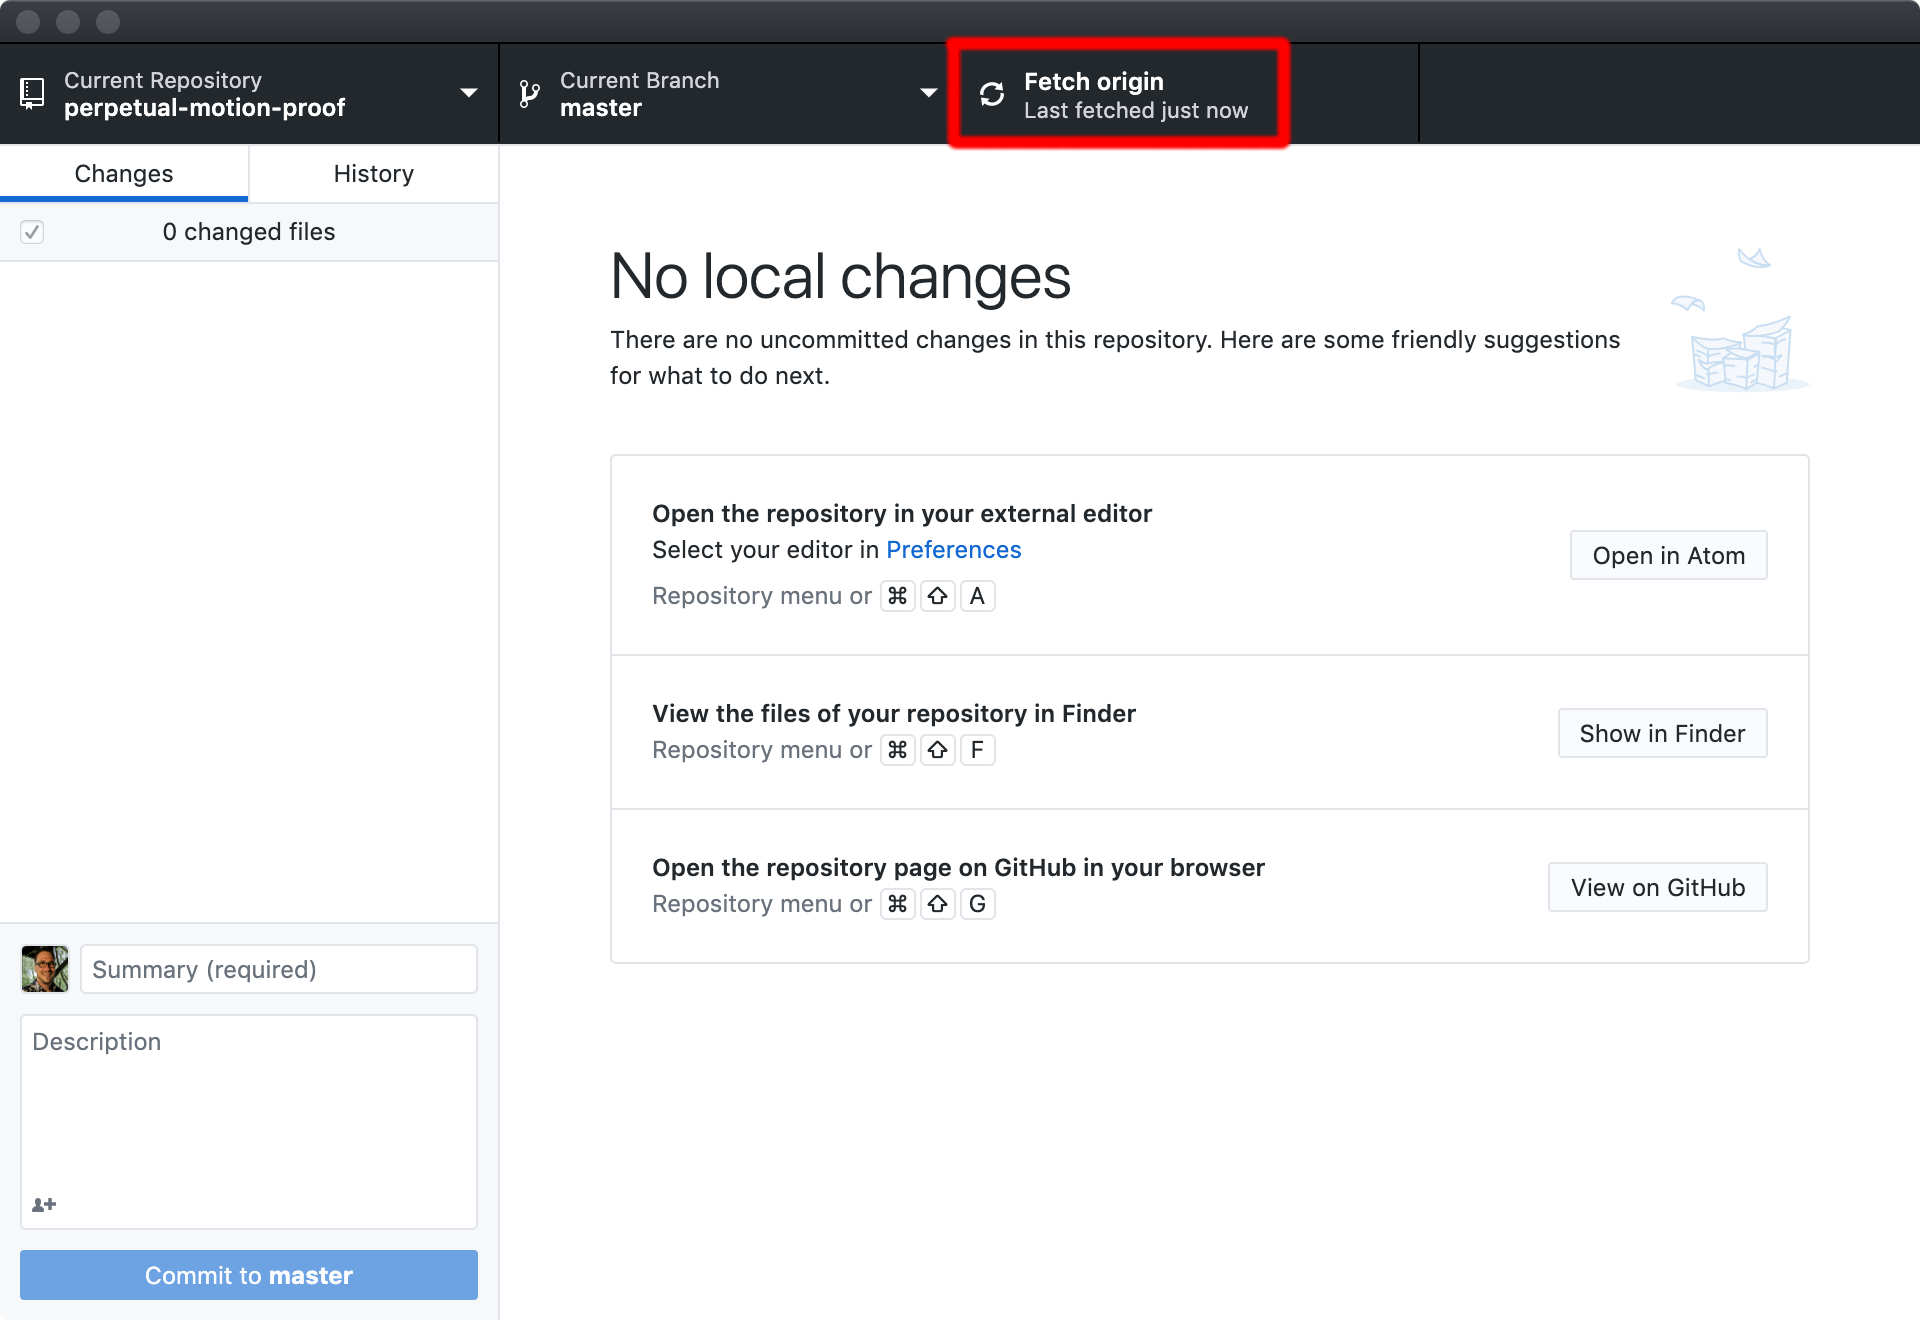
\includegraphics[width=\textwidth]{figures/pull_1.png}
            \end{figure}

            \column{0.5\textwidth}
            \begin{figure}
                \centering
                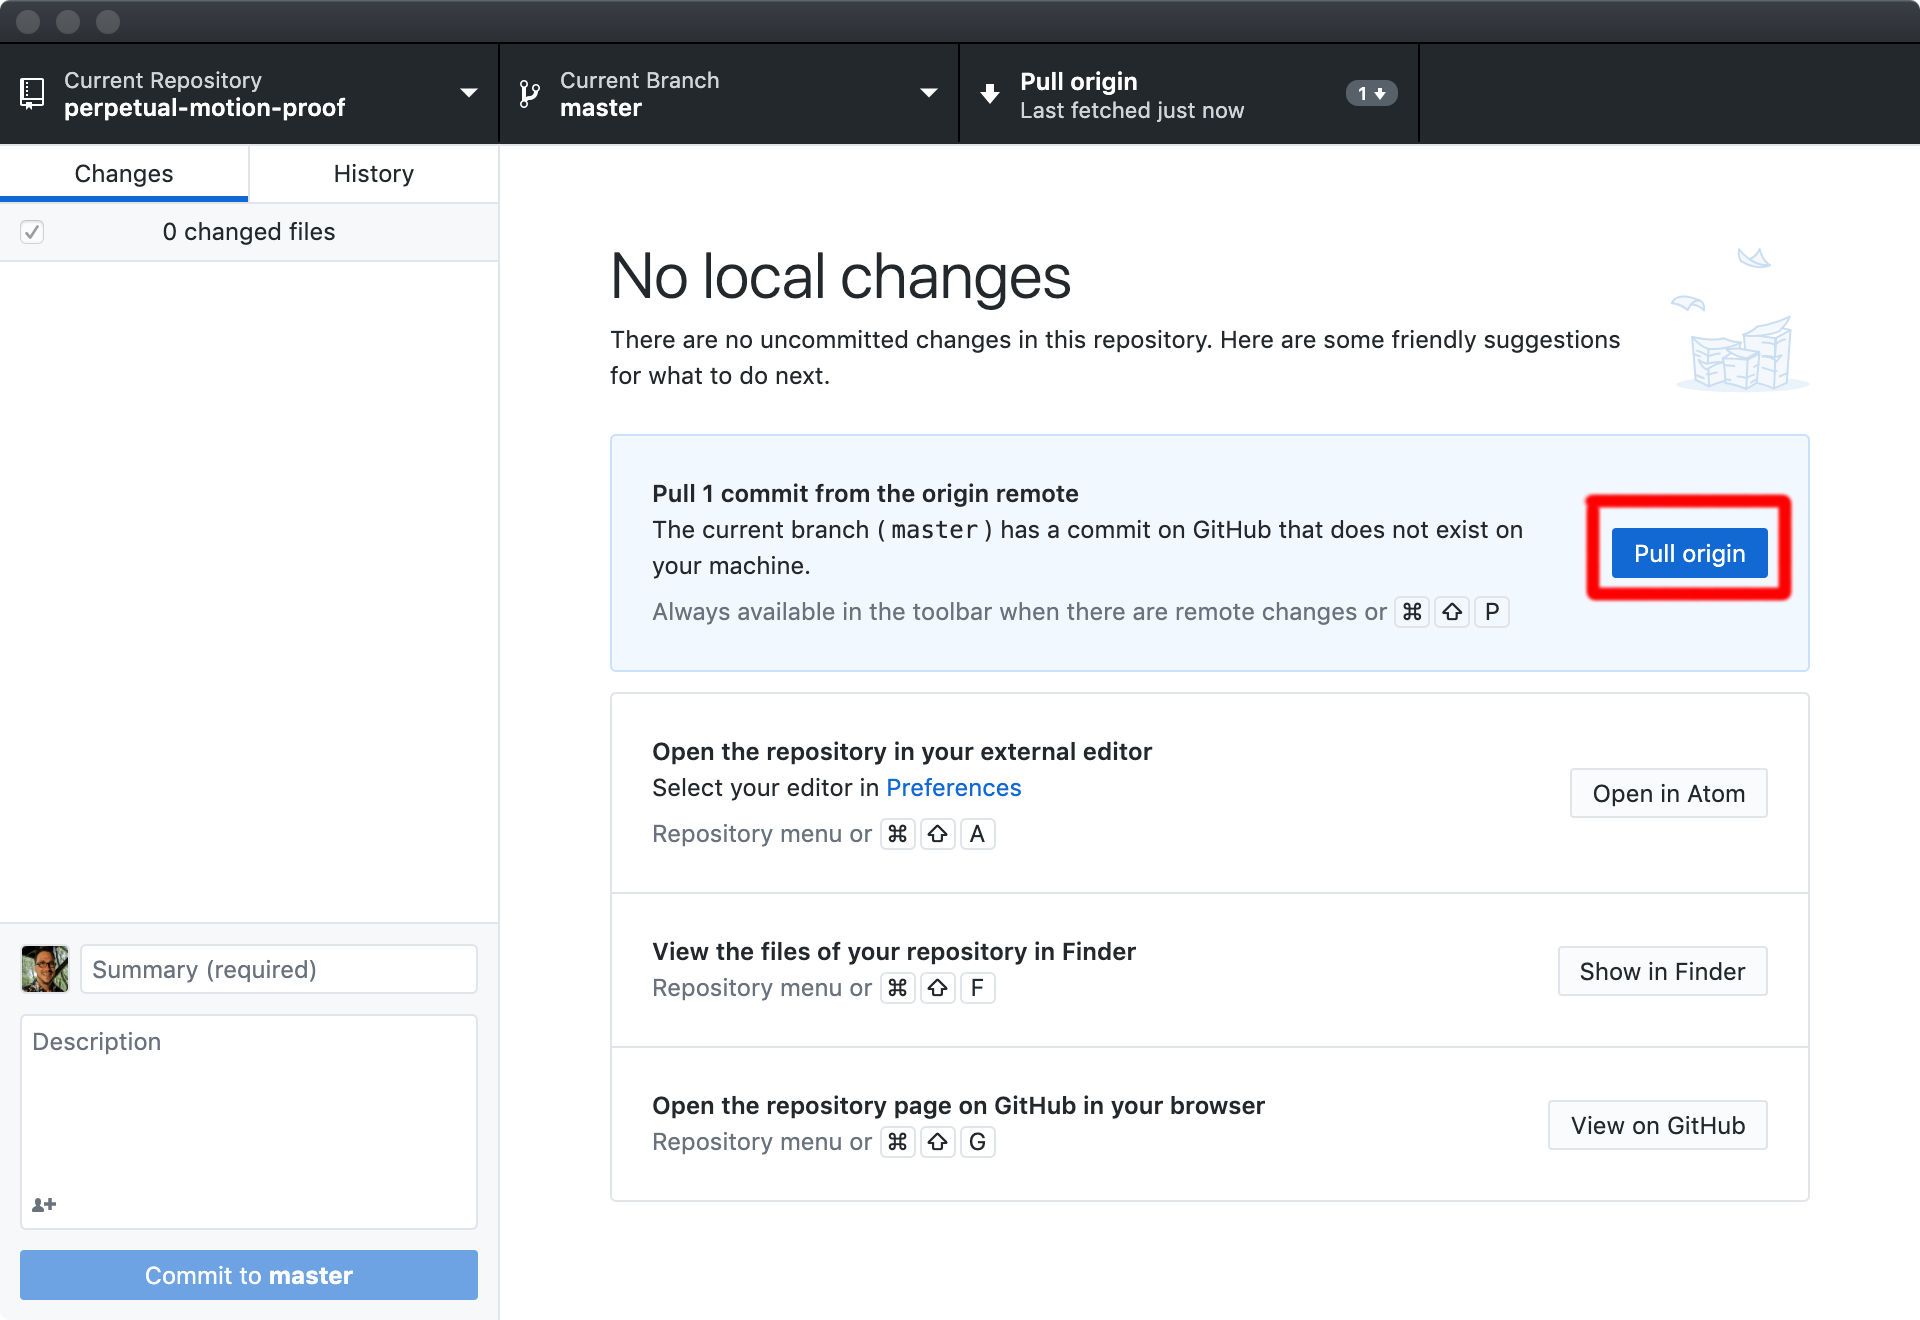
\includegraphics[width=\textwidth]{figures/pull_2.png}
            \end{figure}
        \end{columns}
    \end{frame}

    \begin{frame}{Going Back in Time}
    \end{frame}

    \begin{frame}{Merge Conflicts}
        Merge conflicts occur when one or more people edit the same file
        \begin{itemize}
            \item Alice and Bob both clone a repo from GitHub
            \item Alice and Bob both make changes locally
            \item Bob pushed his changes before Alice
            \item Alice tries to push her changes, but runs into a merge conflict with Bob's changes!
        \end{itemize}
        Before Alice can push her changes, she needs to pull Bob's changes and merge them with her own.
    \end{frame}

    \begin{frame}{Merge Conflicts}
        \begin{figure}
            \centering
            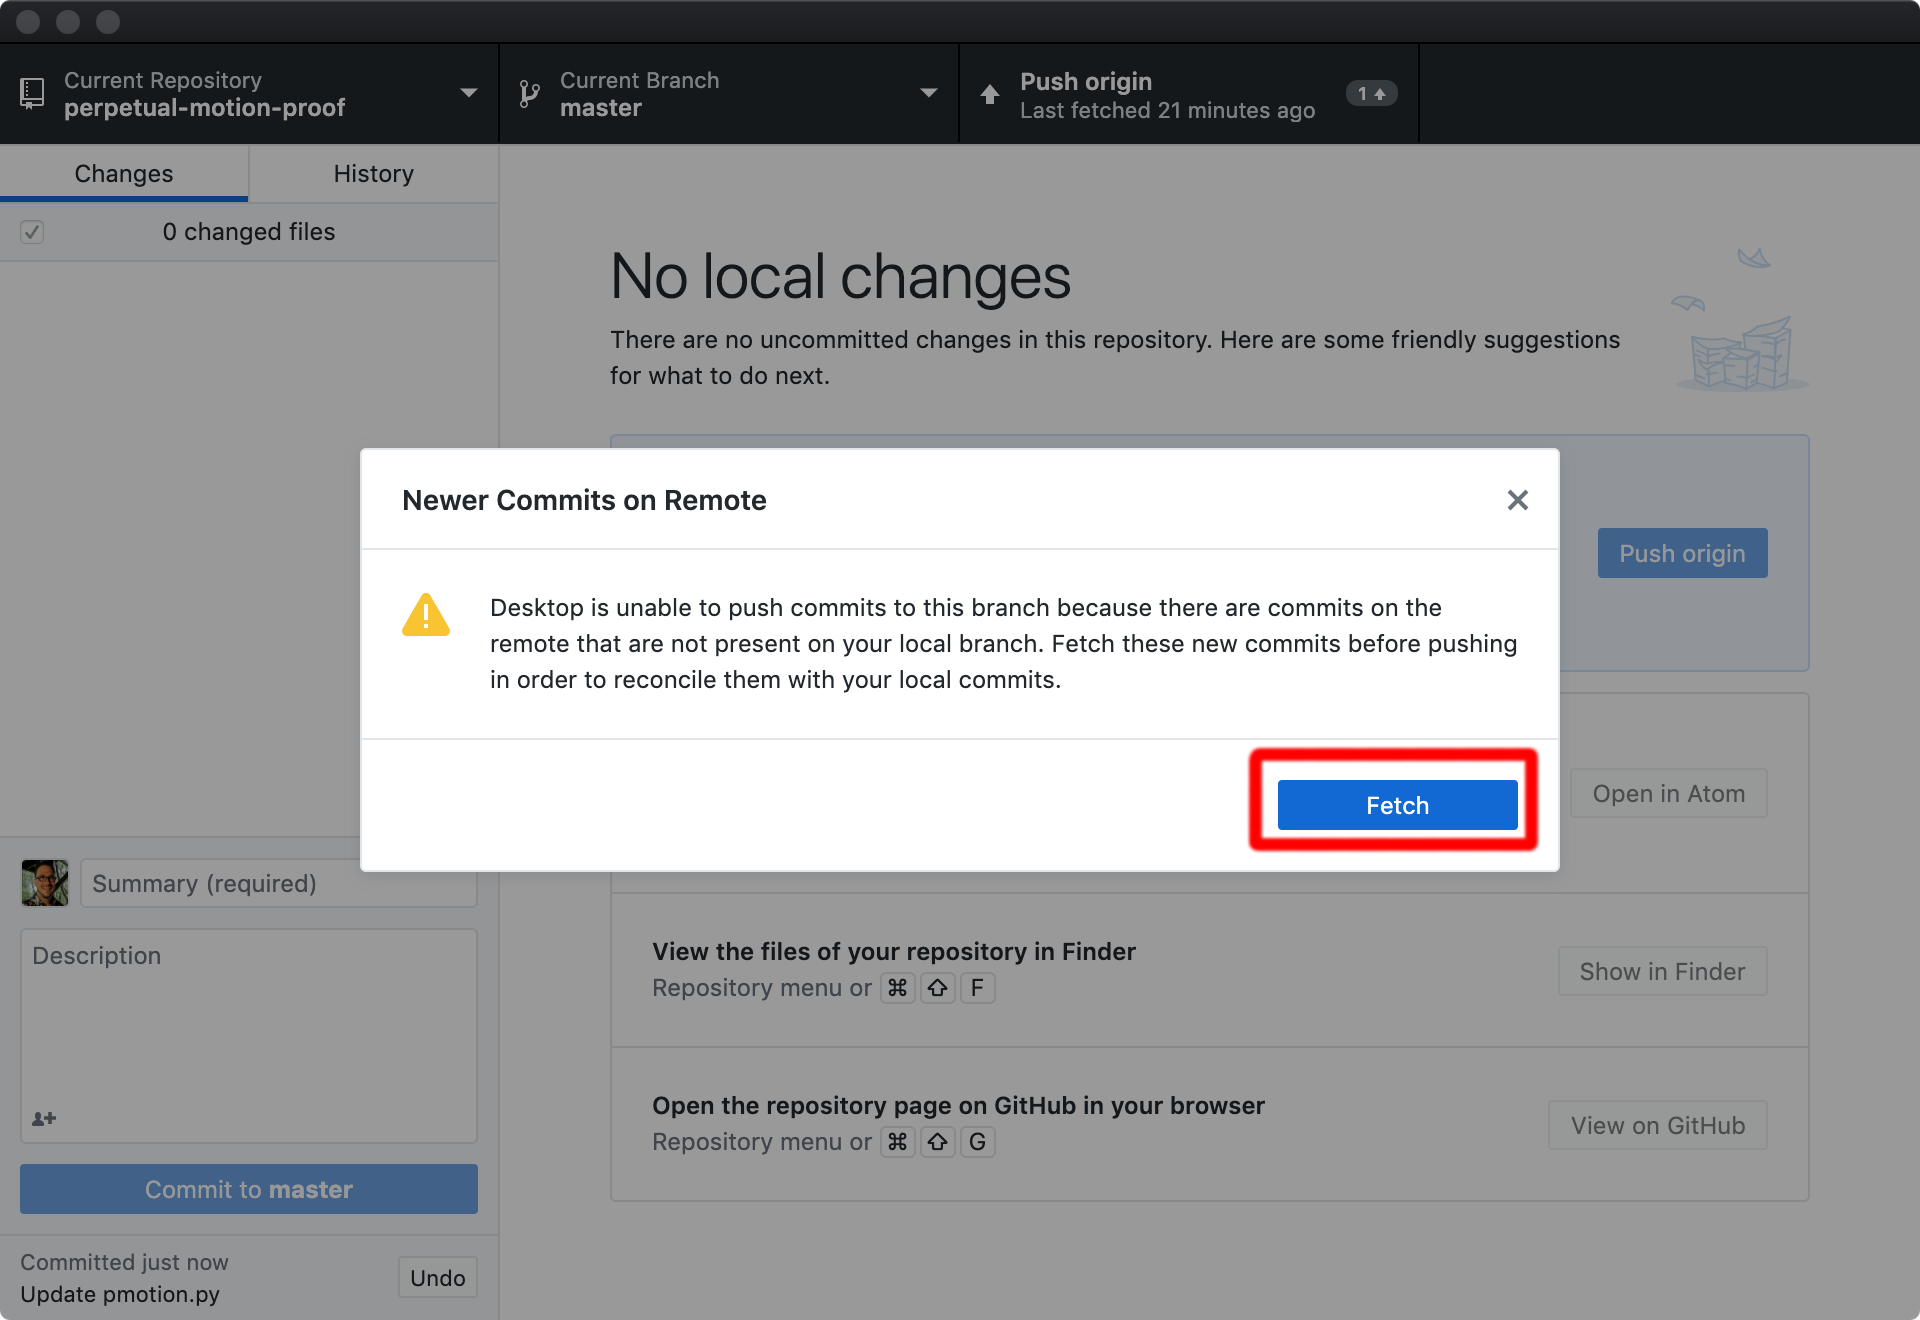
\includegraphics[width=\textwidth]{figures/merge_1.png}
        \end{figure}
    \end{frame}

    \section{Repository Strategies}
    \begin{frame}{A Single Repository}

    \end{frame}

    \begin{frame}{Forking}
    \end{frame}

    \begin{frame}{Branching}
    \end{frame}

    \section{Other Tips}
    \begin{frame}{.gitignore}
        In general, the following items should not be stored in a repository
        \begin{itemize}
            \item Binary files (data files)
            \item Sensitive information
            \item Build files
            \item IDE files
        \end{itemize}
    \end{frame}

    \begin{frame}{.gitignore}
        \begin{figure}
            \centering
            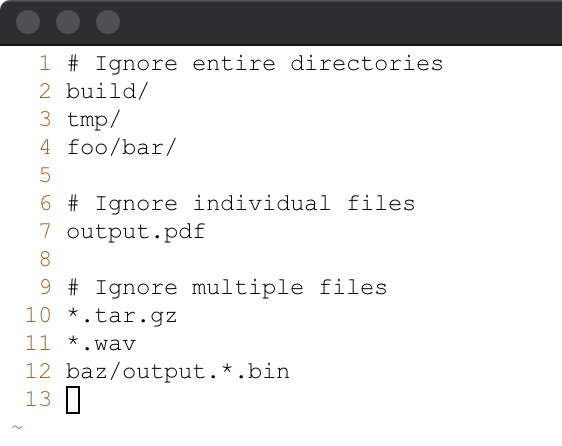
\includegraphics[width=0.7\textwidth]{figures/gitignore.png}
        \end{figure}
        \centering
        Create a file called ``.gitignore" in your repository root
    \end{frame}

    \begin{frame}{Private Repositories}
    \end{frame}

    \section{Project Management}
    \begin{frame}{Project Management}
    \end{frame}

    \section{Resources}
    \begin{frame}{Resources}
    \end{frame}

    \begin{frame}{Thank You!}
        \centering
        Questions?

        \href{mailto:anthony.christe@gmail.com}{anthony.christe@gmail.com}
    \end{frame}


\end{document}